\documentclass[11pt]{article}
\usepackage[T1]{fontenc}
\usepackage[utf8]{inputenc}
\usepackage[margin=2.2cm]{geometry}
\usepackage{amsmath,amssymb,booktabs,longtable,graphicx,xcolor}
\usepackage[hidelinks]{hyperref}
\usepackage{natbib}
\graphicspath{{figures/}{../figures/}}
\setlength{\emergencystretch}{2em}
% generated by src/paper_numbers.py - do not edit by hand
\newcommand{\BAGap}{0.33}
\newcommand{\BARankShare}{84\%}
\newcommand{\BARecRank}{49\%}
\newcommand{\BBdedAUC}{0.823}
\newcommand{\BBdedFone}{59.15}
\newcommand{\BBexact}{850}
\newcommand{\BBfinal}{14{,}041}
\newcommand{\BBgroupAUC}{0.687}
\newcommand{\BBlosoAUC}{0.791}
\newcommand{\BBlosoMax}{0.911}
\newcommand{\BBlosoMin}{0.651}
\newcommand{\BBlosoN}{20}
\newcommand{\BBnPub}{19}
\newcommand{\BBrateMax}{66\%}
\newcommand{\BBrateMin}{7\%}
\newcommand{\BBraw}{15{,}056}
\newcommand{\BBrelAUC}{0.834}
\newcommand{\BBrelAcc}{77.72}
\newcommand{\BBrelFone}{64.37}
\newcommand{\BBrelSVMFone}{63.79}
\newcommand{\BBrelTCFone}{61.29}
\newcommand{\BBseedAUC}{0.821}
\newcommand{\BBseedAUCsd}{0.011}
\newcommand{\BBseedFone}{0.620}
\newcommand{\CellsBelowHalf}{19\%}
\newcommand{\DGEANN}{0.632}
\newcommand{\DGEANNDelta}{$-$0.028}
\newcommand{\DGEANNP}{=0.384}
\newcommand{\DGENDEF}{0.643}
\newcommand{\DGENDEFDelta}{$-$0.018}
\newcommand{\DGENDEFP}{=0.683}
\newcommand{\DGERMlr}{0.660}
\newcommand{\DGERMmlp}{0.639}
\newcommand{\DGERMmlpDelta}{$-$0.021}
\newcommand{\DGERMmlpP}{=0.384}
\newcommand{\DGMDFEND}{0.614}
\newcommand{\DGMDFENDDelta}{$-$0.046}
\newcommand{\DGMDFENDP}{=0.070}
\newcommand{\DGrecEM}{$-$221\%}
\newcommand{\DefPPRErr}{0.34}
\newcommand{\DupIW}{18}
\newcommand{\DupPT}{58}
\newcommand{\DupPTs}{128}
\newcommand{\ECEem}{0.476}
\newcommand{\ECEin}{0.046}
\newcommand{\ECEout}{0.328}
\newcommand{\EMgainPriorRho}{0.19}
\newcommand{\EMpriorErr}{0.46}
\newcommand{\ErrACC}{0.41}
\newcommand{\ErrEMvar}{0.46}
\newcommand{\ErrSrcPPR}{0.12}
\newcommand{\FTInAUC}{0.867}
\newcommand{\FTOffAUC}{0.559}
\newcommand{\FTOffFdef}{0.418}
\newcommand{\FTOffForc}{0.571}
\newcommand{\FTPairAUC}{0.614}
\newcommand{\FTRankShare}{59\%}
\newcommand{\FTRecEM}{$-$51\%}
\newcommand{\FTRecRank}{77\%}
\newcommand{\FTbetterCells}{23}
\newcommand{\FTminusLRin}{$-$0.025}
\newcommand{\FTminusLRoff}{+0.001}
\newcommand{\FTminusLRp}{0.98}
\newcommand{\FTseeds}{3}
\newcommand{\FTsubInAUC}{0.892}
\newcommand{\FTsubOffAUC}{0.558}
\newcommand{\FTsubOffFdef}{0.462}
\newcommand{\FTsubOffForc}{0.566}
\newcommand{\FTsubPairAUC}{0.601}
\newcommand{\GCconflict}{356}
\newcommand{\GCexact}{1{,}174}
\newcommand{\GapOther}{0.44}
\newcommand{\GapPair}{0.31}
\newcommand{\GloveInAUC}{0.864}
\newcommand{\GloveOffAUC}{0.564}
\newcommand{\GroupGC}{0.807}
\newcommand{\GroupLIAR}{0.664}
\newcommand{\GroupPF}{0.840}
\newcommand{\GroupPHEME}{0.644}
\newcommand{\INLPaccAfter}{0.25}
\newcommand{\INLPaccBefore}{0.87}
\newcommand{\ISOTfiv}{6{,}098}
\newcommand{\ISOTreuters}{20{,}768}
\newcommand{\ISOTreutersReal}{20{,}761}
\newcommand{\InAUC}{0.914}
\newcommand{\InAUCmax}{0.914}
\newcommand{\InAUCmin}{0.864}
\newcommand{\InFone}{0.854}
\newcommand{\LCsixfourGC}{0.610}
\newcommand{\LCsixfourISOT}{0.983}
\newcommand{\LCsixfourLIAR}{0.567}
\newcommand{\LCsixfourWEL}{0.894}
\newcommand{\LLMFdef}{0.364}
\newcommand{\LLMFhalf}{0.610}
\newcommand{\LLMForc}{0.638}
\newcommand{\LLMFpm}{0.622}
\newcommand{\LLMauc}{0.657}
\newcommand{\LLMaucMax}{0.730}
\newcommand{\LLMaucMin}{0.574}
\newcommand{\LLMbetterTargets}{7}
\newcommand{\LLMgainMax}{0.13}
\newcommand{\LLMgainMin}{0.06}
\newcommand{\LLMitems}{4{,}532}
\newcommand{\LLMminusLR}{+0.099}
\newcommand{\LLMminusLRp}{9.5e-7}
\newcommand{\LLMppr}{0\%}
\newcommand{\LLMrankShare}{41\%}
\newcommand{\LLMrecHalf}{90\%}
\newcommand{\LocoBal}{0.659}
\newcommand{\LocoBalDelta}{-0.001}
\newcommand{\LocoBalP}{=1.000}
\newcommand{\LocoBestSingle}{0.671}
\newcommand{\LocoCORAL}{0.621}
\newcommand{\LocoCORALDelta}{-0.038}
\newcommand{\LocoCORALP}{<0.001}
\newcommand{\LocoCeiling}{0.914}
\newcommand{\LocoDrop}{0.636}
\newcommand{\LocoDropDelta}{-0.023}
\newcommand{\LocoDropP}{=0.006}
\newcommand{\LocoINLP}{0.605}
\newcommand{\LocoINLPDelta}{-0.054}
\newcommand{\LocoINLPP}{=0.001}
\newcommand{\LocoMask}{0.661}
\newcommand{\LocoMaskDelta}{+0.001}
\newcommand{\LocoMaskP}{=1.000}
\newcommand{\LocoMeanSingle}{0.567}
\newcommand{\LocoPooled}{0.660}
\newcommand{\LocoSVD}{0.647}
\newcommand{\LocoSVDDelta}{-0.013}
\newcommand{\LocoSVDP}{=0.043}
\newcommand{\MaskISOTAllIn}{0.996}
\newcommand{\MaskISOTAllPair}{0.650}
\newcommand{\MaskISOTEntsIn}{0.996}
\newcommand{\MaskISOTEntsPair}{0.657}
\newcommand{\MaskISOTNoneIn}{0.998}
\newcommand{\MaskISOTNonePair}{0.679}
\newcommand{\MaskISOTSourceIn}{0.997}
\newcommand{\MaskISOTSourcePair}{0.681}
\newcommand{\MaskISOTTimeIn}{0.998}
\newcommand{\MaskISOTTimePair}{0.692}
\newcommand{\MaskWELAllIn}{0.964}
\newcommand{\MaskWELAllPair}{0.810}
\newcommand{\MaskWELEntsIn}{0.965}
\newcommand{\MaskWELEntsPair}{0.833}
\newcommand{\MaskWELNoneIn}{0.980}
\newcommand{\MaskWELNonePair}{0.808}
\newcommand{\MaskWELSourceIn}{0.979}
\newcommand{\MaskWELSourcePair}{0.815}
\newcommand{\MaskWELTimeIn}{0.977}
\newcommand{\MaskWELTimePair}{0.831}
\newcommand{\MatchedInAUC}{0.861}
\newcommand{\MatchedOffAUC}{0.556}
\newcommand{\McFracSig}{\textsc{glove-lr} 36\%, \textsc{nb-svm} 21\%, \textsc{roberta-lr} 17\%, \textsc{style-gb} 47\%, \textsc{tfidf-svm} 12\%}
\newcommand{\NcellsBelowHalf}{8}
\newcommand{\Ntotal}{144{,}550}
\newcommand{\OPDef}{0.439}
\newcommand{\OPEM}{0.358}
\newcommand{\OPGMM}{0.510}
\newcommand{\OPHalf}{0.539}
\newcommand{\OPOracle}{0.565}
\newcommand{\OPPrior}{0.547}
\newcommand{\OPRank}{0.541}
\newcommand{\OffAUC}{0.567}
\newcommand{\OffAUCmax}{0.567}
\newcommand{\OffAUCmin}{0.547}
\newcommand{\OffFone}{0.439}
\newcommand{\OffFoneOracle}{0.565}
\newcommand{\OpShareAll}{30\%}
\newcommand{\OpShareOther}{32\%}
\newcommand{\OpSharePair}{21\%}
\newcommand{\OracleCF}{0.537}
\newcommand{\OracleCFbias}{0.028}
\newcommand{\OracleCFbiasSmall}{0.056}
\newcommand{\PADiw}{1.45}
\newcommand{\PADmax}{1.98}
\newcommand{\PADmin}{1.28}
\newcommand{\PADrho}{-0.01}
\newcommand{\PADrhoCI}{[-0.61, 0.69]}
\newcommand{\PSaccRecZero}{$-$32\%}
\newcommand{\PSemRecMax}{$-$43\%}
\newcommand{\PSgainMax}{0.11}
\newcommand{\PSgainMin}{0.02}
\newcommand{\PSrankMinus}{0.477}
\newcommand{\PSrankPlus}{0.491}
\newcommand{\PSrankZero}{0.548}
\newcommand{\PSrecMinus}{58\%}
\newcommand{\PSrecPlus}{22\%}
\newcommand{\PSrecZero}{81\%}
\newcommand{\PStrueMinus}{0.536}
\newcommand{\PStruePlus}{0.541}
\newcommand{\PairAUC}{0.624}
\newcommand{\PairedInAUC}{0.892}
\newcommand{\PermAUC}{0.502}
\newcommand{\PermAUCsd}{0.067}
\newcommand{\PermInAUC}{0.514}
\newcommand{\PriorOther}{0.12}
\newcommand{\PriorPair}{0.05}
\newcommand{\PromiseGapOther}{0.44}
\newcommand{\PromiseGapPair}{0.31}
\newcommand{\PvIsotEmpty}{447}
\newcommand{\PvIsotExact}{5{,}795}
\newcommand{\PvIsotFurther}{270}
\newcommand{\PvIsotFurtherTitle}{267}
\newcommand{\PvIsotRel}{44{,}898}
\newcommand{\PvIsotWork}{38{,}833}
\newcommand{\PvWelAfter}{24{,}540}
\newcommand{\PvWelExact}{8{,}458}
\newcommand{\PvWelExtra}{10}
\newcommand{\PvWelIsotText}{38{,}656}
\newcommand{\PvWelIsotTitle}{480}
\newcommand{\PvWelMD}{73c9675a4b3d09f86a6933d0b8d7d908}
\newcommand{\PvWelOne}{37{,}106}
\newcommand{\PvWelRel}{72{,}134}
\newcommand{\PvWelWork}{24{,}530}
\newcommand{\PvWelZero}{35{,}028}
\newcommand{\RankOther}{0.30}
\newcommand{\RankPair}{0.24}
\newcommand{\RankShareAll}{70\%}
\newcommand{\RankShareCF}{76\%}
\newcommand{\RankShareCI}{[63\%, 79\%]}
\newcommand{\RankShareDropMax}{72\%}
\newcommand{\RankShareDropMin}{67\%}
\newcommand{\RankShareOther}{68\%}
\newcommand{\RankSharePair}{79\%}
\newcommand{\RankWorseShare}{10\%}
\newcommand{\RecACC}{$-$27\%}
\newcommand{\RecEM}{$-$64\%}
\newcommand{\RecEMCI}{[$-$154\%, $-$27\%]}
\newcommand{\RecEMMax}{$-$41\%}
\newcommand{\RecEMMin}{$-$87\%}
\newcommand{\RecGMM}{57\%}
\newcommand{\RecHalf}{80\%}
\newcommand{\RecPrior}{86\%}
\newcommand{\RecPriorCI}{[64\%, 96\%]}
\newcommand{\RecRank}{81\%}
\newcommand{\RecRankCF}{104\%}
\newcommand{\RecRankCI}{[56\%, 91\%]}
\newcommand{\RecRankMax}{81\%}
\newcommand{\RecRankMin}{66\%}
\newcommand{\RecSrcPPR}{76\%}
\newcommand{\RobBetterCells}{17}
\newcommand{\RobInAUC}{0.861}
\newcommand{\RobMinusLRoff}{$-$0.005}
\newcommand{\RobMinusLRp}{0.44}
\newcommand{\RobOffAUC}{0.544}
\newcommand{\RobOffAUCsd}{0.008}
\newcommand{\RobOffFdef}{0.452}
\newcommand{\RobOffForc}{0.549}
\newcommand{\SlackFone}{0.014}
\newcommand{\SlackFoneMax}{0.037}
\newcommand{\SrcPriorErr}{0.09}
\newcommand{\StyleISOT}{0.999}
\newcommand{\StyleInAUC}{0.745}
\newcommand{\StyleOffAUC}{0.535}
\newcommand{\StyleShare}{57\%}
\newcommand{\StyleWEL}{0.951}
\newcommand{\SubLRInAUC}{0.895}
\newcommand{\SubLROffAUC}{0.549}
\newcommand{\SubLROffAUCsd}{0.008}
\newcommand{\SubLROffFdef}{0.435}
\newcommand{\SubLROffForc}{0.560}
\newcommand{\ThrOther}{0.02}
\newcommand{\ThrPair}{0.02}
\newcommand{\TopKISOTIn}{0.999}
\newcommand{\TopKISOTInMax}{0.985}
\newcommand{\TopKISOTInThousand}{0.991}
\newcommand{\TopKISOTPair}{0.673}
\newcommand{\TopKISOTPairMax}{0.580}
\newcommand{\TopKISOTPairThousand}{0.597}
\newcommand{\TopKWELIn}{0.984}
\newcommand{\TopKWELInMax}{0.949}
\newcommand{\TopKWELInThousand}{0.962}
\newcommand{\TopKWELPair}{0.827}
\newcommand{\TopKWELPairMax}{0.718}
\newcommand{\TopKWELPairThousand}{0.754}
\newcommand{\TopicGCBalIn}{0.799}
\newcommand{\TopicGCBalOut}{0.519}
\newcommand{\TopicGCDropped}{61\%}
\newcommand{\TopicGCPurity}{0.76}
\newcommand{\TopicGCRandIn}{0.846}
\newcommand{\TopicGCRandOut}{0.542}
\newcommand{\TopicISOTBalIn}{0.999}
\newcommand{\TopicISOTBalOut}{0.606}
\newcommand{\TopicISOTDropped}{65\%}
\newcommand{\TopicISOTPurity}{0.82}
\newcommand{\TopicISOTRandIn}{0.998}
\newcommand{\TopicISOTRandOut}{0.604}
\newcommand{\TopicLIARBalIn}{0.687}
\newcommand{\TopicLIARBalOut}{0.532}
\newcommand{\TopicLIARDropped}{21\%}
\newcommand{\TopicLIARPurity}{0.63}
\newcommand{\TopicLIARRandIn}{0.692}
\newcommand{\TopicLIARRandOut}{0.530}
\newcommand{\TopicWELBalIn}{0.986}
\newcommand{\TopicWELBalOut}{0.622}
\newcommand{\TopicWELDropped}{50\%}
\newcommand{\TopicWELPurity}{0.81}
\newcommand{\TopicWELRandIn}{0.984}
\newcommand{\TopicWELRandOut}{0.622}
\newcommand{\TwShared}{169}
\newcommand{\WELfiv}{125}
\newcommand{\WELnear}{815}
\newcommand{\WELnyt}{6{,}223}
\newcommand{\WELrelFiv}{6{,}261}
\newcommand{\WELrelNyt}{6{,}223}
\newcommand{\WELrelReu}{21{,}270}
\newcommand{\WELrelReuN}{21{,}289}
\newcommand{\XlBBEN}{0.777}
\newcommand{\XlBBtoEN}{0.931}
\newcommand{\XlBN}{0.813}
\newcommand{\XlEN}{0.994}
\newcommand{\XlENtoBB}{0.707}
\newcommand{\XlTransCost}{0.04}
\newcommand{\pairGCPFAUC}{0.59}
\newcommand{\pairGCPFCI}{[0.50, 0.68]}
\newcommand{\pairGCPFFdef}{0.425}
\newcommand{\pairGCPFForc}{0.595}
\newcommand{\pairGCPFFpm}{0.576}
\newcommand{\pairGCPFIn}{0.869}
\newcommand{\pairGCPFPPR}{0.07}
\newcommand{\pairGCPFPrior}{0.43}
\newcommand{\pairISOTWELFakeAUC}{0.69}
\newcommand{\pairISOTWELFakeCI}{[0.66, 0.71]}
\newcommand{\pairISOTWELFakeFdef}{0.539}
\newcommand{\pairISOTWELFakeForc}{0.638}
\newcommand{\pairISOTWELFakeFpm}{0.635}
\newcommand{\pairISOTWELFakeIn}{0.999}
\newcommand{\pairISOTWELFakePPR}{0.78}
\newcommand{\pairISOTWELFakePrior}{0.43}
\newcommand{\pairLIARPFAUC}{0.51}
\newcommand{\pairLIARPFCI}{[0.42, 0.60]}
\newcommand{\pairLIARPFFdef}{0.495}
\newcommand{\pairLIARPFForc}{0.536}
\newcommand{\pairLIARPFFpm}{0.517}
\newcommand{\pairLIARPFIn}{0.698}
\newcommand{\pairLIARPFPPR}{0.54}
\newcommand{\pairLIARPFPrior}{0.44}
\newcommand{\pairPFGCAUC}{0.53}
\newcommand{\pairPFGCCI}{[0.48, 0.56]}
\newcommand{\pairPFGCFdef}{0.464}
\newcommand{\pairPFGCForc}{0.517}
\newcommand{\pairPFGCFpm}{0.514}
\newcommand{\pairPFGCIn}{0.893}
\newcommand{\pairPFGCPPR}{0.54}
\newcommand{\pairPFGCPrior}{0.23}
\newcommand{\pairPFLIARAUC}{0.50}
\newcommand{\pairPFLIARCI}{[0.47, 0.54]}
\newcommand{\pairPFLIARFdef}{0.497}
\newcommand{\pairPFLIARForc}{0.509}
\newcommand{\pairPFLIARFpm}{0.502}
\newcommand{\pairPFLIARIn}{0.893}
\newcommand{\pairPFLIARPPR}{0.40}
\newcommand{\pairPFLIARPrior}{0.44}
\newcommand{\pairTwATwBAUC}{0.67}
\newcommand{\pairTwATwBCI}{[0.52, 0.82]}
\newcommand{\pairTwATwBFdef}{0.572}
\newcommand{\pairTwATwBForc}{0.646}
\newcommand{\pairTwATwBFpm}{0.597}
\newcommand{\pairTwATwBIn}{0.981}
\newcommand{\pairTwATwBPPR}{0.62}
\newcommand{\pairTwATwBPrior}{0.46}
\newcommand{\pairTwBTwAAUC}{0.66}
\newcommand{\pairTwBTwACI}{[0.55, 0.75]}
\newcommand{\pairTwBTwAFdef}{0.580}
\newcommand{\pairTwBTwAForc}{0.631}
\newcommand{\pairTwBTwAFpm}{0.591}
\newcommand{\pairTwBTwAIn}{0.967}
\newcommand{\pairTwBTwAPPR}{0.63}
\newcommand{\pairTwBTwAPrior}{0.51}
\newcommand{\pairWELFakeISOTAUC}{0.85}
\newcommand{\pairWELFakeISOTCI}{[0.82, 0.87]}
\newcommand{\pairWELFakeISOTFdef}{0.753}
\newcommand{\pairWELFakeISOTForc}{0.765}
\newcommand{\pairWELFakeISOTFpm}{0.763}
\newcommand{\pairWELFakeISOTIn}{0.989}
\newcommand{\pairWELFakeISOTPPR}{0.36}
\newcommand{\pairWELFakeISOTPrior}{0.46}

\renewcommand{\thetable}{S\arabic{table}}
\renewcommand{\thefigure}{S\arabic{figure}}
\renewcommand{\thesection}{S\arabic{section}}

\title{Supplementary Material\\[4pt]\large Mostly ranking, partly threshold: decomposing and repairing the cross-corpus generalisation gap of misinformation detectors}
\author{Dewan Fahad Chowdhury\thanks{Equal contribution, joint first authors.} \and Md.\ Rejaul Korim Sadi\footnotemark[1]\\[2pt]
\small Department of Computer Science and Engineering, Metropolitan University, Sylhet, Bangladesh}
\date{}

\begin{document}
\maketitle

\noindent This supplement documents how the data were prepared and how every number in the paper was produced. All tables here are written by \texttt{src/paper\_numbers.py} from the result files released with the code; the repository's \texttt{run\_all.sh} regenerates them end to end.

\section{Data preparation}
\subsection{Label harmonisation and verification}
Every corpus is mapped to $1=$ fake, false, rumour or clickbait. The WELFake release codes $1=$ fake although its record documents $0=$ fake, $1=$ real; our working copy followed the documented legend and is inverted back; LIAR keeps \{pants-fire, false\} versus \{mostly-true, true\}; Twitter15/16 keep false versus true. Label direction was verified on the raw files with outlet signatures (\texttt{src/label\_probe.py}): Table~\ref{tab:probe}.
\begin{table}[h]
\centering
\caption{Label-direction probes: number of items matching each source signature under raw label 0 / raw label 1 (``copy'' is our working copy of WELFake). A reliable-outlet signature should sit under ``real'' and a fake-site signature under ``fake''. ISOT and the WELFake release both code $1=$ fake (although the WELFake record's legend says $0=$ fake); the WELFake working copy, made by following that legend, has every label inverted.}\label{tab:probe}
\footnotesize
\begin{tabular}{@{}llrrr@{}}
\toprule
Signature & Expected & ISOT & WELFake release & WELFake copy \\
\midrule
title ends '- The New York Times' & real & 0 / 0 & 6{,}223 / 0 & 0 / 6{,}223 \\
title ends '- Breitbart' & real & 0 / 0 & 2{,}338 / 2 & 1 / 2{,}338 \\
text contains '(Reuters)' & real & 20{,}761 / 7 & 21{,}270 / 19 & 8 / 23 \\
text contains 'Featured image via' & fake & 0 / 6{,}098 & 0 / 6{,}261 & 125 / 0 \\
title contains 'BREAKING' & fake & 8 / 614 & 28 / 1{,}154 & 199 / 19 \\
text contains '21st Century Wire' & fake & 0 / 629 & 0 / 1{,}272 & 5 / 0 \\
text contains 'Activist Post' & fake & 0 / 5 & 0 / 33 & 21 / 0 \\
\bottomrule
\end{tabular}
\end{table}


\subsection{Deduplication}
Within each corpus, rows are normalised (NFKC, lower case, URLs and punctuation removed), exact duplicates are removed, and near-duplicates are clustered with MinHash-LSH (128 permutations, Jaccard $\geq 0.8$; word 3-grams over the first 400 words for articles, character 5-grams otherwise). Any exact or near-duplicate group whose members disagree on the label is removed entirely; otherwise one member is kept. Across corpora, each item is flagged with the corpora in which it has a near-duplicate, and transfer tests drop flagged target items.
\begin{table}[h]
\centering
\caption{Deduplication report per corpus.}\label{tab:supp-dedup}
\small
\begin{tabular}{@{}lrrrrrrr@{}}
\toprule
Corpus & raw & empty & exact conflict & exact dup. & near conflict & near dup. & final \\
\midrule
ISOT & 38{,}833 & 5 & 0 & 0 & 0 & 79 & 38{,}749 \\
WELFake & 24{,}530 & 1 & 0 & 0 & 6 & 815 & 23{,}708 \\
PolitiFact & 1{,}056 & 0 & 4 & 71 & 2 & 3 & 976 \\
GossipCop & 22{,}140 & 0 & 356 & 1{,}174 & 24 & 26 & 20{,}560 \\
LIAR & 8{,}090 & 0 & 3 & 21 & 0 & 11 & 8{,}055 \\
Twitter15 & 742 & 0 & 0 & 55 & 0 & 14 & 673 \\
Twitter16 & 412 & 0 & 0 & 51 & 0 & 3 & 358 \\
PHEME & 5{,}802 & 0 & 21 & 124 & 4 & 98 & 5{,}555 \\
ClickbaitEN & 32{,}000 & 0 & 0 & 2 & 0 & 123 & 31{,}875 \\
BanglaBait & 15{,}056 & 0 & 23 & 850 & 18 & 124 & 14{,}041 \\
\bottomrule
\end{tabular}
\end{table}


\section{Evaluation details}
Splits are stratified 70/10/20 per seed (0--4), with caps of 8{,}000/1{,}500/3{,}000 items. Hyperparameters are chosen on the source validation split by ROC-AUC, and scores are Platt-calibrated on the same split. Metrics are computed on the target test split after near-duplicate exclusion. Pooled seed-bootstrap intervals use 200 resamples per seed, pooled across seeds. Operating points: default $t=0.5$; EM prior adaptation \citep{saerens2002adjusting} with 200 iterations and tolerance $10^{-6}$; rate transfer (threshold at the $(1-\pi_A)$ quantile of the target scores); 0.5-rate (median threshold); a 2-component Gaussian mixture on target logits; the true-prior quantile; adjusted classify-and-count \citep{forman2008quantifying} with error rates from the source test split at $t=0.5$ (falling back to the raw flag rate when $\mathrm{TPR}-\mathrm{FPR}<0.05$, estimates clipped to $[0.01,0.99]$); the source in-domain flag rate $q_A$; and the oracle maximum over 199 quantile thresholds. The cross-fitted oracle tunes the threshold on a random half of the target test set and scores it on the other half, for five random splits and both halves. Corpus-bootstrap intervals resample the seven veracity corpora with replacement (2{,}000 draws, seed 0) and weight each directed pair of distinct drawn corpora by the product of their multiplicities. The prior-shift experiment resamples each target test set with replacement to 1{,}000 items at base rate $\pi_A+\delta$, $\delta\in\{-0.3,-0.2,\dots,0.3\}$, clipped to $[0.05,0.95]$, three draws per cell and seed.

\paragraph{Fine-tuned RoBERTa}
Weights: RoBERTa-base as packaged in spaCy \texttt{en\_core\_web\_trf} 3.8.0 (byte-level BPE, 12 layers). The embedding layer and layers 1--8 are frozen; their output for every text is computed once (16-bit floats) and cached. Layers 9--12 and a linear head on the mask-weighted mean of the final states are trained with AdamW (weight decay 0.01, learning rate $3\times10^{-5}$ for the layers and $10^{-3}$ for the head, linear decay, gradient clipping at 1.0), batch size 16, three epochs, binary cross-entropy with positive-class weight $(1-\pi_A)/\pi_A$, dropout 0.1. The epoch with the highest validation AUC is kept and its scores are Platt-calibrated on validation. Inputs are the first 1{,}500 characters, cut to 128 word pieces for articles and 64 for the other units. Each source uses 800 training and 200 validation items and each target 300 test items, stratified subsets of the seed's regular splits, for seeds 0--2. The paired \textsc{tfidf-lr} sees the first 600 characters of the same items.
\begin{table}[h]
\centering
\caption{Share of the operating-point loss (oracle minus default macro-F1, off-diagonal cells) recovered by each threshold rule, per detector. Rate rules flag the top share of target items given by the source base rate $\pi_A$, the source in-domain flag rate $q_A$, one half, the adjusted classify-and-count estimate (ACC), or the true target base rate. The last two columns give the mean absolute error of the ACC and EM estimates of the target base rate; the source base rate itself is off by 0.09 on average.}\label{tab:supp-rates}
\footnotesize
\begin{tabular}{@{}lrrrrrrrrrrr@{}}
\toprule
Model & F1$_{0.5}$ & F1$^\star$ & EM & $\pi_A$ & $q_A$ & 0.5 & ACC & GMM & $\pi_B$ & err.\ ACC & err.\ EM \\
\midrule
\textsc{tfidf-lr} & 0.439 & 0.565 & $-$64\% & 81\% & 76\% & 80\% & $-$27\% & 57\% & 86\% & 0.41 & 0.46 \\
\textsc{tfidf-svm} & 0.437 & 0.564 & $-$59\% & 81\% & 77\% & 79\% & $-$29\% & 52\% & 86\% & 0.42 & 0.45 \\
\textsc{nb-svm} & 0.410 & 0.555 & $-$41\% & 79\% & 76\% & 80\% & $-$16\% & 24\% & 85\% & 0.44 & 0.48 \\
\textsc{glove-lr} & 0.465 & 0.564 & $-$84\% & 76\% & 65\% & 78\% & $-$56\% & 29\% & 83\% & 0.41 & 0.43 \\
\textsc{style-gb} & 0.427 & 0.548 & $-$67\% & 77\% & 64\% & 77\% & $-$36\% & 41\% & 84\% & 0.43 & 0.46 \\
\textsc{roberta-lr} & 0.452 & 0.549 & $-$87\% & 66\% & 52\% & 66\% & $-$49\% & 25\% & 75\% & 0.39 & 0.43 \\
\textsc{roberta-ft} & 0.418 & 0.571 & $-$51\% & 77\% & 67\% & 76\% & $-$23\% & 40\% & 82\% & 0.42 & 0.48 \\
\bottomrule
\end{tabular}
\end{table}


\section{Exact values behind the main-text figures}
The main text shows these results as figures; the tables below give the exact values.
\begin{table}[t]
\centering
\caption{In-domain versus transfer performance on the seven veracity corpora (mean $\pm$ s.d.\ over seeds of the per-seed mean over cells). ``Pairs'' averages the eight directed same-task cells. Off-diagonal macro-F1 is given at the default threshold and at the oracle threshold. \textsc{roberta-lr} is evaluated on the 1{,}500-item subsets and \textsc{roberta-ft} on 800 training and 300 test items per corpus with three seeds (Section~\ref{sec:models}); compare each with its paired \textsc{tfidf-lr} in Section~\ref{sec:models-res}, not with the rows above.}\label{tab:headline}
\small
\setlength{\tabcolsep}{4pt}
\begin{tabular}{@{}llcccccc@{}}
\toprule
 & & \multicolumn{3}{c}{ROC-AUC} & \multicolumn{3}{c}{macro-F1} \\
\cmidrule(lr){3-5}\cmidrule(lr){6-8}
Model & Regime & In-domain & Off-diag. & Pairs & In-domain & Off-diag. & Off-diag.\ oracle \\
\midrule
\textsc{tfidf-lr} & full & 0.914\,{\scriptsize$\pm$0.006} & 0.567\,{\scriptsize$\pm$0.006} & 0.624\,{\scriptsize$\pm$0.004} & 0.854\,{\scriptsize$\pm$0.005} & 0.439\,{\scriptsize$\pm$0.011} & 0.565\,{\scriptsize$\pm$0.004} \\
\textsc{tfidf-lr} & matched & 0.861\,{\scriptsize$\pm$0.010} & 0.556\,{\scriptsize$\pm$0.004} & 0.590\,{\scriptsize$\pm$0.009} & 0.786\,{\scriptsize$\pm$0.012} & 0.446\,{\scriptsize$\pm$0.014} & 0.558\,{\scriptsize$\pm$0.002} \\
\textsc{tfidf-lr} & permuted & 0.519\,{\scriptsize$\pm$0.026} & 0.499\,{\scriptsize$\pm$0.012} & 0.514\,{\scriptsize$\pm$0.019} & 0.397\,{\scriptsize$\pm$0.014} & 0.377\,{\scriptsize$\pm$0.015} & 0.518\,{\scriptsize$\pm$0.007} \\
\addlinespace
\textsc{tfidf-svm} & full & 0.914\,{\scriptsize$\pm$0.005} & 0.564\,{\scriptsize$\pm$0.005} & 0.625\,{\scriptsize$\pm$0.005} & 0.855\,{\scriptsize$\pm$0.005} & 0.437\,{\scriptsize$\pm$0.009} & 0.564\,{\scriptsize$\pm$0.004} \\
\textsc{tfidf-svm} & matched & 0.862\,{\scriptsize$\pm$0.010} & 0.554\,{\scriptsize$\pm$0.005} & 0.592\,{\scriptsize$\pm$0.010} & 0.787\,{\scriptsize$\pm$0.011} & 0.447\,{\scriptsize$\pm$0.017} & 0.556\,{\scriptsize$\pm$0.003} \\
\textsc{tfidf-svm} & permuted & 0.519\,{\scriptsize$\pm$0.024} & 0.498\,{\scriptsize$\pm$0.015} & 0.511\,{\scriptsize$\pm$0.020} & 0.398\,{\scriptsize$\pm$0.009} & 0.377\,{\scriptsize$\pm$0.012} & 0.516\,{\scriptsize$\pm$0.008} \\
\addlinespace
\textsc{nb-svm} & full & 0.912\,{\scriptsize$\pm$0.004} & 0.547\,{\scriptsize$\pm$0.006} & 0.590\,{\scriptsize$\pm$0.011} & 0.853\,{\scriptsize$\pm$0.008} & 0.410\,{\scriptsize$\pm$0.008} & 0.555\,{\scriptsize$\pm$0.003} \\
\textsc{nb-svm} & matched & 0.862\,{\scriptsize$\pm$0.011} & 0.540\,{\scriptsize$\pm$0.006} & 0.559\,{\scriptsize$\pm$0.004} & 0.786\,{\scriptsize$\pm$0.012} & 0.398\,{\scriptsize$\pm$0.013} & 0.549\,{\scriptsize$\pm$0.004} \\
\textsc{nb-svm} & permuted & 0.510\,{\scriptsize$\pm$0.023} & 0.494\,{\scriptsize$\pm$0.009} & 0.502\,{\scriptsize$\pm$0.009} & 0.400\,{\scriptsize$\pm$0.003} & 0.383\,{\scriptsize$\pm$0.012} & 0.520\,{\scriptsize$\pm$0.006} \\
\addlinespace
\textsc{glove-lr} & full & 0.864\,{\scriptsize$\pm$0.005} & 0.564\,{\scriptsize$\pm$0.005} & 0.610\,{\scriptsize$\pm$0.005} & 0.782\,{\scriptsize$\pm$0.007} & 0.465\,{\scriptsize$\pm$0.004} & 0.564\,{\scriptsize$\pm$0.004} \\
\textsc{glove-lr} & matched & 0.830\,{\scriptsize$\pm$0.006} & 0.563\,{\scriptsize$\pm$0.010} & 0.592\,{\scriptsize$\pm$0.017} & 0.740\,{\scriptsize$\pm$0.011} & 0.466\,{\scriptsize$\pm$0.010} & 0.564\,{\scriptsize$\pm$0.007} \\
\textsc{glove-lr} & permuted & 0.520\,{\scriptsize$\pm$0.022} & 0.504\,{\scriptsize$\pm$0.026} & 0.494\,{\scriptsize$\pm$0.021} & 0.404\,{\scriptsize$\pm$0.020} & 0.391\,{\scriptsize$\pm$0.012} & 0.525\,{\scriptsize$\pm$0.019} \\
\addlinespace
\textsc{style-gb} & full & 0.745\,{\scriptsize$\pm$0.009} & 0.535\,{\scriptsize$\pm$0.004} & 0.595\,{\scriptsize$\pm$0.008} & 0.679\,{\scriptsize$\pm$0.005} & 0.427\,{\scriptsize$\pm$0.007} & 0.548\,{\scriptsize$\pm$0.003} \\
\textsc{style-gb} & matched & 0.702\,{\scriptsize$\pm$0.008} & 0.526\,{\scriptsize$\pm$0.009} & 0.561\,{\scriptsize$\pm$0.032} & 0.632\,{\scriptsize$\pm$0.008} & 0.413\,{\scriptsize$\pm$0.017} & 0.542\,{\scriptsize$\pm$0.007} \\
\textsc{style-gb} & permuted & 0.503\,{\scriptsize$\pm$0.018} & 0.502\,{\scriptsize$\pm$0.016} & 0.493\,{\scriptsize$\pm$0.028} & 0.410\,{\scriptsize$\pm$0.008} & 0.390\,{\scriptsize$\pm$0.007} & 0.523\,{\scriptsize$\pm$0.011} \\
\addlinespace
\textsc{roberta-lr} & full & 0.861\,{\scriptsize$\pm$0.012} & 0.544\,{\scriptsize$\pm$0.008} & 0.630\,{\scriptsize$\pm$0.011} & 0.777\,{\scriptsize$\pm$0.013} & 0.452\,{\scriptsize$\pm$0.013} & 0.549\,{\scriptsize$\pm$0.010} \\
\addlinespace
\textsc{roberta-ft} & full & 0.867\,{\scriptsize$\pm$0.010} & 0.559\,{\scriptsize$\pm$0.013} & 0.614\,{\scriptsize$\pm$0.020} & 0.795\,{\scriptsize$\pm$0.005} & 0.418\,{\scriptsize$\pm$0.009} & 0.571\,{\scriptsize$\pm$0.008} \\
\bottomrule
\end{tabular}
\end{table}

\begin{table}[t]
\centering
\caption{Same-task pairs (\textsc{tfidf-lr}, five seeds). AUC with pooled seed-bootstrap 95\% CI; ``In'' is the source's in-domain AUC; prior is the target fake rate and PPR the predicted-positive rate at $t=0.5$; macro-F1 at the default, prior-matched and oracle thresholds; ECE of the source-calibrated scores on the target.}\label{tab:pairs}
\small
\begin{tabular}{@{}lcccccccc@{}}
\toprule
Pair & In & AUC [95\% CI] & Prior & PPR & F1$_{0.5}$ & F1$_{\pi}$ & F1$^\star$ & ECE \\
\midrule
ISOT$\to$WELFake & 0.999 & 0.690 [0.66, 0.71] & 0.43 & 0.78 & 0.539 & 0.635 & 0.638 & 0.38 \\
WELFake$\to$ISOT & 0.989 & 0.847 [0.82, 0.87] & 0.46 & 0.36 & 0.753 & 0.763 & 0.765 & 0.11 \\
PolitiFact$\to$GossipCop & 0.893 & 0.526 [0.48, 0.56] & 0.23 & 0.54 & 0.464 & 0.514 & 0.517 & 0.32 \\
GossipCop$\to$PolitiFact & 0.869 & 0.589 [0.50, 0.68] & 0.43 & 0.07 & 0.425 & 0.576 & 0.595 & 0.28 \\
Twitter15$\to$Twitter16 & 0.981 & 0.672 [0.52, 0.82] & 0.46 & 0.62 & 0.572 & 0.597 & 0.646 & 0.25 \\
Twitter16$\to$Twitter15 & 0.967 & 0.657 [0.55, 0.75] & 0.51 & 0.63 & 0.580 & 0.591 & 0.631 & 0.28 \\
LIAR$\to$PolitiFact & 0.698 & 0.508 [0.42, 0.60] & 0.44 & 0.54 & 0.495 & 0.517 & 0.536 & 0.12 \\
PolitiFact$\to$LIAR & 0.893 & 0.505 [0.47, 0.54] & 0.44 & 0.40 & 0.497 & 0.502 & 0.509 & 0.22 \\
\bottomrule
\end{tabular}
\end{table}

\begin{table}[t]
\centering
\caption{Transfer gap decomposition (Eq.~\ref{eq:decomp}), macro-F1 points, mean over cells and seeds. The gap is relative to the target's own in-domain score.}\label{tab:decomp}
\small
\begin{tabular}{@{}llrrrrr@{}}
\toprule
Model & Cells & Gap & Ranking & Threshold & Prior/cal. & Ranking share \\
\midrule
\textsc{tfidf-lr} & pairs & 0.308 & 0.244 & 0.018 & 0.046 & 79\% \\
\textsc{tfidf-lr} & other cells & 0.441 & 0.300 & 0.018 & 0.122 & 68\% \\
\textsc{tfidf-svm} & pairs & 0.308 & 0.243 & 0.016 & 0.049 & 79\% \\
\textsc{tfidf-svm} & other cells & 0.444 & 0.303 & 0.018 & 0.123 & 68\% \\
\textsc{nb-svm} & pairs & 0.319 & 0.261 & 0.023 & 0.036 & 82\% \\
\textsc{nb-svm} & other cells & 0.472 & 0.306 & 0.021 & 0.145 & 65\% \\
\textsc{glove-lr} & pairs & 0.281 & 0.193 & 0.016 & 0.071 & 69\% \\
\textsc{glove-lr} & other cells & 0.327 & 0.224 & 0.017 & 0.085 & 69\% \\
\textsc{style-gb} & pairs & 0.141 & 0.091 & 0.013 & 0.036 & 65\% \\
\textsc{style-gb} & other cells & 0.278 & 0.141 & 0.020 & 0.117 & 51\% \\
\textsc{roberta-lr} & pairs & 0.243 & 0.162 & 0.022 & 0.059 & 66\% \\
\textsc{roberta-lr} & other cells & 0.344 & 0.244 & 0.024 & 0.076 & 71\% \\
\textsc{roberta-ft} & pairs & 0.340 & 0.186 & 0.031 & 0.123 & 55\% \\
\textsc{roberta-ft} & other cells & 0.387 & 0.233 & 0.027 & 0.127 & 60\% \\
\bottomrule
\end{tabular}
\end{table}

\begin{table}[t]
\centering
\caption{Off-diagonal macro-F1 under different operating points (mean over the 42 cells and five seeds). Label-free: default $t=0.5$, EM prior adaptation, rate transfer (predicted-positive rate set to the source base rate), predicted-positive rate 0.5, and a 2-component GMM on target logits. With one number known: rate set to the true target prior. Upper bound: oracle threshold. For \textsc{tfidf-lr}, Holm-corrected Wilcoxon $p$ versus default: EM 1.6e-32, rate transfer 6.6e-31, rate 0.5 1.4e-29, GMM 1.7e-18.}\label{tab:oppoints}
\small
\begin{tabular}{@{}lccccccc@{}}
\toprule
 & \multicolumn{5}{c}{label-free} & prior known & bound \\
\cmidrule(lr){2-6}\cmidrule(lr){7-7}\cmidrule(lr){8-8}
Model & $t=0.5$ & EM & rate transfer & rate 0.5 & GMM & rate $=\pi_B$ & oracle \\
\midrule
\textsc{tfidf-lr} & 0.439 & 0.358 & 0.541 & 0.539 & 0.510 & 0.547 & 0.565 \\
\textsc{tfidf-svm} & 0.437 & 0.363 & 0.539 & 0.537 & 0.503 & 0.546 & 0.564 \\
\textsc{nb-svm} & 0.410 & 0.349 & 0.525 & 0.526 & 0.444 & 0.534 & 0.555 \\
\textsc{glove-lr} & 0.465 & 0.381 & 0.540 & 0.542 & 0.494 & 0.547 & 0.564 \\
\textsc{style-gb} & 0.427 & 0.347 & 0.521 & 0.521 & 0.477 & 0.529 & 0.548 \\
\textsc{roberta-lr} & 0.452 & 0.368 & 0.516 & 0.516 & 0.477 & 0.525 & 0.549 \\
\textsc{roberta-ft} & 0.418 & 0.340 & 0.535 & 0.534 & 0.479 & 0.544 & 0.571 \\
\bottomrule
\end{tabular}
\end{table}

\begin{table}[t]
\centering
\caption{Shortcut indicators (ROC-AUC, mean of five seeds). In-domain AUC of \textsc{tfidf-lr} with the full training split, of the surface-statistics \textsc{style-gb}, and of \textsc{tfidf-lr} trained on only 64 or 256 items; AUC of a group-identity baseline (publisher domain for PolitiFact and GossipCop, speaker for LIAR); and the mean off-diagonal AUC with the corpus as source and as target.}\label{tab:shortcuts}
\small
\begin{tabular}{@{}lccccccc@{}}
\toprule
 & \multicolumn{5}{c}{in-domain} & \multicolumn{2}{c}{transfer} \\
\cmidrule(lr){2-6}\cmidrule(lr){7-8}
Corpus & full & style only & $n=64$ & $n=256$ & group only & as source & as target \\
\midrule
ISOT & 0.999 & 0.999 & 0.983 & 0.991 & -- & 0.611 & 0.670 \\
WELFake & 0.989 & 0.951 & 0.894 & 0.941 & -- & 0.626 & 0.540 \\
PolitiFact & 0.893 & 0.787 & 0.742 & 0.850 & 0.840 & 0.533 & 0.592 \\
GossipCop & 0.869 & 0.659 & 0.610 & 0.723 & 0.807 & 0.538 & 0.522 \\
LIAR & 0.698 & 0.590 & 0.567 & 0.607 & 0.664 & 0.537 & 0.530 \\
Twitter15 & 0.981 & 0.603 & 0.793 & 0.962 & -- & 0.572 & 0.563 \\
Twitter16 & 0.967 & 0.625 & 0.890 & -- & -- & 0.556 & 0.552 \\
\bottomrule
\end{tabular}
\end{table}

\begin{table}[t]
\centering
\caption{Masking ablation (\textsc{tfidf-lr}, ROC-AUC, three seeds, first 3{,}000 characters). Rows: training corpus and what is masked in every corpus; columns: test corpus (the training corpus's own column is in-domain).}\label{tab:mask}
\small
\begin{tabular}{@{}llccccc@{}}
\toprule
Train & Masked & ISOT & WELFake & PolitiFact & GossipCop & LIAR \\
\midrule
ISOT & none & 0.998 & 0.679 & 0.739 & 0.481 & 0.559 \\
ISOT & source tags, datelines, URLs, handles & 0.997 & 0.681 & 0.733 & 0.483 & 0.559 \\
ISOT & dates, weekdays, numbers & 0.998 & 0.692 & 0.723 & 0.479 & 0.563 \\
ISOT & named entities & 0.996 & 0.657 & 0.678 & 0.543 & 0.557 \\
ISOT & all of the above & 0.996 & 0.650 & 0.678 & 0.540 & 0.556 \\
\addlinespace
WELFake & none & 0.808 & 0.980 & 0.636 & 0.529 & 0.532 \\
WELFake & source tags, datelines, URLs, handles & 0.815 & 0.979 & 0.634 & 0.533 & 0.536 \\
WELFake & dates, weekdays, numbers & 0.831 & 0.977 & 0.608 & 0.509 & 0.526 \\
WELFake & named entities & 0.833 & 0.965 & 0.614 & 0.511 & 0.522 \\
WELFake & all of the above & 0.810 & 0.964 & 0.611 & 0.500 & 0.522 \\
\bottomrule
\end{tabular}
\end{table}

\begin{table}[t]
\centering
\caption{Leave-one-corpus-out repairs (\textsc{tfidf-lr} features; mean over the seven held-out veracity corpora and five seeds; s.d.\ across seeds). $\Delta$AUC versus pooled training with Holm-corrected Wilcoxon $p$ over the 35 (target, seed) pairs. For reference, the mean single-source transfer AUC to the same targets is 0.567, the best single source (chosen with target labels) 0.671, and the targets' own in-domain AUC 0.914.}\label{tab:repair}
\small
\begin{tabular}{@{}lccccc@{}}
\toprule
Training & AUC & AP & F1$_{0.5}$ & F1$^\star$ & $\Delta$AUC ($p$) \\
\midrule
pooled (6 corpora) & 0.660\,{\scriptsize$\pm$0.013} & 0.582 & 0.581 & 0.634 & -- \\
+ (corpus, class) balancing & 0.659\,{\scriptsize$\pm$0.013} & 0.583 & 0.582 & 0.632 & -0.001 (1.000) \\
+ balancing + masking & 0.661\,{\scriptsize$\pm$0.012} & 0.584 & 0.576 & 0.633 & +0.001 (1.000) \\
+ balancing + corpus-feature deletion & 0.636\,{\scriptsize$\pm$0.011} & 0.556 & 0.560 & 0.611 & -0.023 (0.006) \\
SVD-300 + balancing & 0.647\,{\scriptsize$\pm$0.009} & 0.566 & 0.583 & 0.624 & -0.013 (0.043) \\
SVD-300 + INLP & 0.605\,{\scriptsize$\pm$0.011} & 0.520 & 0.525 & 0.591 & -0.054 (0.001) \\
SVD-300 + CORAL & 0.621\,{\scriptsize$\pm$0.008} & 0.539 & 0.563 & 0.604 & -0.038 ($<$0.001) \\
\bottomrule
\end{tabular}
\end{table}

\begin{table}[h]
\centering
\caption{Leave-one-corpus-out AUC per held-out corpus (mean of five seeds), against single-source transfer and the in-domain ceiling.}\label{tab:repair-targets}
\small
\begin{tabular}{@{}lccccccc@{}}
\toprule
Held out & mean single & best single & pooled & + masking & INLP & CORAL & in-domain \\
\midrule
ISOT & 0.670 & 0.847 & 0.865 & 0.890 & 0.805 & 0.781 & 0.999 \\
WELFake & 0.540 & 0.690 & 0.648 & 0.657 & 0.643 & 0.643 & 0.989 \\
PolitiFact & 0.592 & 0.730 & 0.677 & 0.655 & 0.600 & 0.650 & 0.893 \\
GossipCop & 0.522 & 0.544 & 0.538 & 0.546 & 0.558 & 0.520 & 0.869 \\
LIAR & 0.530 & 0.552 & 0.528 & 0.528 & 0.502 & 0.514 & 0.698 \\
Twitter15 & 0.563 & 0.657 & 0.647 & 0.645 & 0.592 & 0.626 & 0.981 \\
Twitter16 & 0.552 & 0.678 & 0.715 & 0.703 & 0.536 & 0.616 & 0.967 \\
\bottomrule
\end{tabular}
\end{table}

\begin{table}[h]
\centering
\caption{Held-out-corpus ROC-AUC of published generalisation methods re-implemented on frozen RoBERTa vectors (leave-one-corpus-out, mean of three seeds).}\label{tab:dg}
\footnotesize
\begin{tabular}{@{}lcccccccc@{}}
\toprule
Method & ISOT & WELFake & PolitiFact & GossipCop & LIAR & Tw15 & Tw16 & Mean \\
\midrule
pooled logistic regression & 0.924 & 0.800 & 0.705 & 0.547 & 0.477 & 0.602 & 0.565 & 0.660 \\
pooled MLP & 0.953 & 0.764 & 0.588 & 0.544 & 0.474 & 0.574 & 0.579 & 0.639 \\
EANN-style adversarial & 0.936 & 0.727 & 0.569 & 0.567 & 0.469 & 0.586 & 0.574 & 0.632 \\
MDFEND-style experts & 0.927 & 0.689 & 0.501 & 0.551 & 0.474 & 0.595 & 0.559 & 0.614 \\
ENDEF-style entity debiasing & 0.942 & 0.760 & 0.592 & 0.556 & 0.474 & 0.581 & 0.594 & 0.643 \\
\bottomrule
\end{tabular}
\end{table}

\begin{table}[t]
\centering
\caption{BanglaBait, official split. Clickbait-class F1, precision and recall and accuracy (\%), as reported by \citet{mahtab2023banglabait}, plus ROC-AUC. Reference values from that paper (as released): LR char 3--5-grams F1 66.28, BanglaBERT 71.72, SS-GAN BanglaBERT 75.13.}\label{tab:bangla}
\small
\begin{tabular}{@{}lllrrrrr@{}}
\toprule
Test set & Input & Model & F1 & P & R & Acc. & AUC \\
\midrule
as released & title & LR, char 3--5 & 64.37 & 73.63 & 57.17 & 77.72 & 0.834 \\
as released & title & SVM, char 3--5 & 63.79 & 73.37 & 56.42 & 77.46 & 0.836 \\
as released & title & LR, word 1--2 & 48.51 & 65.59 & 38.49 & 71.25 & 0.737 \\
as released & title+content & LR, char 3--5 & 61.29 & 71.92 & 53.40 & 76.26 & 0.792 \\
as released & title+content & SVM, char 3--5 & 60.68 & 71.78 & 52.55 & 76.03 & 0.791 \\
as released & title+content & LR, word 1--2 & 57.48 & 70.36 & 48.58 & 74.70 & 0.775 \\
\addlinespace
deduplicated & title & LR, char 3--5 & 59.15 & 70.72 & 50.84 & 76.57 & 0.823 \\
deduplicated & title & SVM, char 3--5 & 60.01 & 71.23 & 51.85 & 76.94 & 0.824 \\
deduplicated & title & LR, word 1--2 & 40.77 & 64.56 & 29.79 & 71.11 & 0.722 \\
deduplicated & title+content & LR, char 3--5 & 52.34 & 67.98 & 42.55 & 74.14 & 0.772 \\
deduplicated & title+content & SVM, char 3--5 & 53.28 & 69.42 & 43.23 & 74.70 & 0.772 \\
deduplicated & title+content & LR, word 1--2 & 48.61 & 66.86 & 38.19 & 73.06 & 0.752 \\
\bottomrule
\end{tabular}
\end{table}

\clearpage
\begin{figure}[h]
\centering
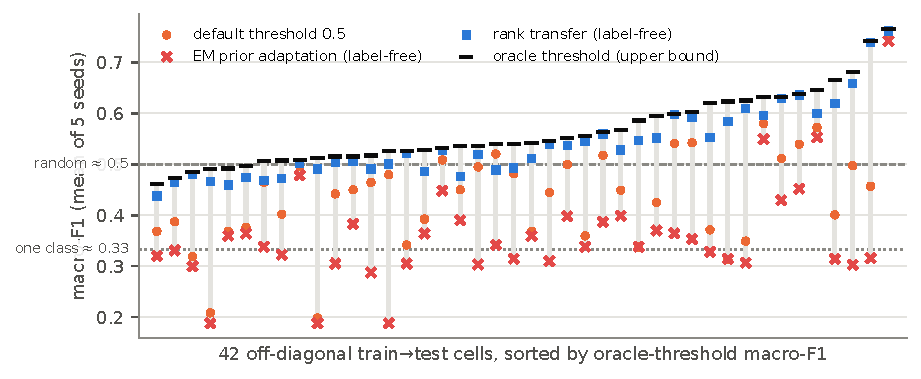
\includegraphics[width=0.95\linewidth]{fig_operating_points}
\caption{Off-diagonal macro-F1 of \textsc{tfidf-lr} for each of the 42 cells (mean of five seeds), sorted by the oracle bound. Rate transfer closes most of the distance from the default threshold to the oracle without any target label; EM prior adaptation often falls below the default.}\label{fig:op}
\end{figure}
\clearpage

\section{Full results}
\subsection{Transfer matrices for every model}
\begin{table}[h]
\centering
\caption{\textsc{tfidf-lr}, ROC-AUC (rows: training corpus; columns: test corpus; mean $\pm$ s.d.\ over five seeds).}
\scriptsize
\begin{tabular}{@{}lccccccc@{}}
\toprule
 & ISOT & WELFake & PolitiFact & GossipCop & LIAR & Tw15 & Tw16 \\
\midrule
ISOT & \textbf{1.00\,{\tiny$\pm$0.00}} & 0.69\,{\tiny$\pm$0.01} & 0.73\,{\tiny$\pm$0.02} & 0.49\,{\tiny$\pm$0.01} & 0.55\,{\tiny$\pm$0.02} & 0.52\,{\tiny$\pm$0.06} & 0.68\,{\tiny$\pm$0.10} \\
WELFake & 0.85\,{\tiny$\pm$0.01} & \textbf{0.99\,{\tiny$\pm$0.00}} & 0.66\,{\tiny$\pm$0.02} & 0.53\,{\tiny$\pm$0.01} & 0.53\,{\tiny$\pm$0.02} & 0.58\,{\tiny$\pm$0.03} & 0.62\,{\tiny$\pm$0.07} \\
PolitiFact & 0.80\,{\tiny$\pm$0.01} & 0.46\,{\tiny$\pm$0.01} & \textbf{0.89\,{\tiny$\pm$0.02}} & 0.53\,{\tiny$\pm$0.02} & 0.50\,{\tiny$\pm$0.01} & 0.51\,{\tiny$\pm$0.04} & 0.39\,{\tiny$\pm$0.04} \\
GossipCop & 0.48\,{\tiny$\pm$0.04} & 0.50\,{\tiny$\pm$0.07} & 0.59\,{\tiny$\pm$0.03} & \textbf{0.87\,{\tiny$\pm$0.01}} & 0.54\,{\tiny$\pm$0.02} & 0.63\,{\tiny$\pm$0.01} & 0.48\,{\tiny$\pm$0.03} \\
LIAR & 0.59\,{\tiny$\pm$0.04} & 0.63\,{\tiny$\pm$0.02} & 0.51\,{\tiny$\pm$0.02} & 0.54\,{\tiny$\pm$0.02} & \textbf{0.70\,{\tiny$\pm$0.01}} & 0.48\,{\tiny$\pm$0.05} & 0.47\,{\tiny$\pm$0.05} \\
Twitter15 & 0.63\,{\tiny$\pm$0.05} & 0.51\,{\tiny$\pm$0.03} & 0.54\,{\tiny$\pm$0.01} & 0.54\,{\tiny$\pm$0.02} & 0.54\,{\tiny$\pm$0.02} & \textbf{0.98\,{\tiny$\pm$0.01}} & 0.67\,{\tiny$\pm$0.05} \\
Twitter16 & 0.68\,{\tiny$\pm$0.03} & 0.46\,{\tiny$\pm$0.01} & 0.53\,{\tiny$\pm$0.04} & 0.51\,{\tiny$\pm$0.00} & 0.51\,{\tiny$\pm$0.02} & 0.66\,{\tiny$\pm$0.03} & \textbf{0.97\,{\tiny$\pm$0.02}} \\
\bottomrule
\end{tabular}
\end{table}

\begin{table}[h]
\centering
\caption{\textsc{tfidf-lr}, macro-F1 at $t=0.5$ (rows: training corpus; columns: test corpus; mean $\pm$ s.d.\ over five seeds).}
\scriptsize
\begin{tabular}{@{}lccccccc@{}}
\toprule
 & ISOT & WELFake & PolitiFact & GossipCop & LIAR & Tw15 & Tw16 \\
\midrule
ISOT & \textbf{0.99\,{\tiny$\pm$0.00}} & 0.54\,{\tiny$\pm$0.01} & 0.50\,{\tiny$\pm$0.03} & 0.21\,{\tiny$\pm$0.01} & 0.44\,{\tiny$\pm$0.03} & 0.36\,{\tiny$\pm$0.03} & 0.40\,{\tiny$\pm$0.06} \\
WELFake & 0.75\,{\tiny$\pm$0.01} & \textbf{0.95\,{\tiny$\pm$0.00}} & 0.35\,{\tiny$\pm$0.03} & 0.20\,{\tiny$\pm$0.00} & 0.34\,{\tiny$\pm$0.01} & 0.34\,{\tiny$\pm$0.00} & 0.31\,{\tiny$\pm$0.00} \\
PolitiFact & 0.46\,{\tiny$\pm$0.03} & 0.32\,{\tiny$\pm$0.01} & \textbf{0.81\,{\tiny$\pm$0.02}} & 0.46\,{\tiny$\pm$0.02} & 0.50\,{\tiny$\pm$0.01} & 0.52\,{\tiny$\pm$0.05} & 0.37\,{\tiny$\pm$0.03} \\
GossipCop & 0.37\,{\tiny$\pm$0.02} & 0.38\,{\tiny$\pm$0.01} & 0.43\,{\tiny$\pm$0.04} & \textbf{0.76\,{\tiny$\pm$0.00}} & 0.37\,{\tiny$\pm$0.01} & 0.37\,{\tiny$\pm$0.02} & 0.39\,{\tiny$\pm$0.05} \\
LIAR & 0.52\,{\tiny$\pm$0.03} & 0.54\,{\tiny$\pm$0.03} & 0.49\,{\tiny$\pm$0.02} & 0.48\,{\tiny$\pm$0.01} & \textbf{0.63\,{\tiny$\pm$0.01}} & 0.46\,{\tiny$\pm$0.03} & 0.48\,{\tiny$\pm$0.05} \\
Twitter15 & 0.54\,{\tiny$\pm$0.05} & 0.44\,{\tiny$\pm$0.03} & 0.50\,{\tiny$\pm$0.03} & 0.45\,{\tiny$\pm$0.06} & 0.51\,{\tiny$\pm$0.03} & \textbf{0.93\,{\tiny$\pm$0.03}} & 0.57\,{\tiny$\pm$0.04} \\
Twitter16 & 0.51\,{\tiny$\pm$0.12} & 0.39\,{\tiny$\pm$0.07} & 0.45\,{\tiny$\pm$0.07} & 0.40\,{\tiny$\pm$0.08} & 0.45\,{\tiny$\pm$0.06} & 0.58\,{\tiny$\pm$0.03} & \textbf{0.92\,{\tiny$\pm$0.03}} \\
\bottomrule
\end{tabular}
\end{table}

\begin{table}[h]
\centering
\caption{\textsc{tfidf-svm}, ROC-AUC (rows: training corpus; columns: test corpus; mean $\pm$ s.d.\ over five seeds).}
\scriptsize
\begin{tabular}{@{}lccccccc@{}}
\toprule
 & ISOT & WELFake & PolitiFact & GossipCop & LIAR & Tw15 & Tw16 \\
\midrule
ISOT & \textbf{1.00\,{\tiny$\pm$0.00}} & 0.72\,{\tiny$\pm$0.01} & 0.71\,{\tiny$\pm$0.02} & 0.50\,{\tiny$\pm$0.02} & 0.55\,{\tiny$\pm$0.01} & 0.52\,{\tiny$\pm$0.07} & 0.68\,{\tiny$\pm$0.10} \\
WELFake & 0.85\,{\tiny$\pm$0.01} & \textbf{0.99\,{\tiny$\pm$0.00}} & 0.66\,{\tiny$\pm$0.02} & 0.52\,{\tiny$\pm$0.02} & 0.53\,{\tiny$\pm$0.02} & 0.56\,{\tiny$\pm$0.03} & 0.61\,{\tiny$\pm$0.06} \\
PolitiFact & 0.80\,{\tiny$\pm$0.02} & 0.45\,{\tiny$\pm$0.02} & \textbf{0.89\,{\tiny$\pm$0.02}} & 0.52\,{\tiny$\pm$0.02} & 0.51\,{\tiny$\pm$0.01} & 0.52\,{\tiny$\pm$0.04} & 0.39\,{\tiny$\pm$0.05} \\
GossipCop & 0.48\,{\tiny$\pm$0.04} & 0.50\,{\tiny$\pm$0.06} & 0.59\,{\tiny$\pm$0.03} & \textbf{0.87\,{\tiny$\pm$0.01}} & 0.54\,{\tiny$\pm$0.02} & 0.63\,{\tiny$\pm$0.00} & 0.48\,{\tiny$\pm$0.04} \\
LIAR & 0.58\,{\tiny$\pm$0.04} & 0.63\,{\tiny$\pm$0.02} & 0.51\,{\tiny$\pm$0.02} & 0.55\,{\tiny$\pm$0.02} & \textbf{0.70\,{\tiny$\pm$0.01}} & 0.49\,{\tiny$\pm$0.03} & 0.47\,{\tiny$\pm$0.05} \\
Twitter15 & 0.58\,{\tiny$\pm$0.06} & 0.50\,{\tiny$\pm$0.04} & 0.52\,{\tiny$\pm$0.01} & 0.53\,{\tiny$\pm$0.02} & 0.54\,{\tiny$\pm$0.02} & \textbf{0.98\,{\tiny$\pm$0.01}} & 0.64\,{\tiny$\pm$0.06} \\
Twitter16 & 0.68\,{\tiny$\pm$0.03} & 0.46\,{\tiny$\pm$0.01} & 0.53\,{\tiny$\pm$0.04} & 0.51\,{\tiny$\pm$0.01} & 0.51\,{\tiny$\pm$0.02} & 0.66\,{\tiny$\pm$0.02} & \textbf{0.96\,{\tiny$\pm$0.01}} \\
\bottomrule
\end{tabular}
\end{table}

\begin{table}[h]
\centering
\caption{\textsc{tfidf-svm}, macro-F1 at $t=0.5$ (rows: training corpus; columns: test corpus; mean $\pm$ s.d.\ over five seeds).}
\scriptsize
\begin{tabular}{@{}lccccccc@{}}
\toprule
 & ISOT & WELFake & PolitiFact & GossipCop & LIAR & Tw15 & Tw16 \\
\midrule
ISOT & \textbf{0.99\,{\tiny$\pm$0.00}} & 0.53\,{\tiny$\pm$0.02} & 0.42\,{\tiny$\pm$0.03} & 0.20\,{\tiny$\pm$0.01} & 0.40\,{\tiny$\pm$0.03} & 0.35\,{\tiny$\pm$0.01} & 0.34\,{\tiny$\pm$0.03} \\
WELFake & 0.77\,{\tiny$\pm$0.01} & \textbf{0.96\,{\tiny$\pm$0.00}} & 0.37\,{\tiny$\pm$0.01} & 0.21\,{\tiny$\pm$0.00} & 0.36\,{\tiny$\pm$0.02} & 0.34\,{\tiny$\pm$0.01} & 0.31\,{\tiny$\pm$0.00} \\
PolitiFact & 0.45\,{\tiny$\pm$0.03} & 0.32\,{\tiny$\pm$0.01} & \textbf{0.81\,{\tiny$\pm$0.03}} & 0.47\,{\tiny$\pm$0.02} & 0.50\,{\tiny$\pm$0.01} & 0.53\,{\tiny$\pm$0.04} & 0.39\,{\tiny$\pm$0.05} \\
GossipCop & 0.37\,{\tiny$\pm$0.02} & 0.37\,{\tiny$\pm$0.01} & 0.41\,{\tiny$\pm$0.03} & \textbf{0.76\,{\tiny$\pm$0.00}} & 0.37\,{\tiny$\pm$0.01} & 0.37\,{\tiny$\pm$0.02} & 0.40\,{\tiny$\pm$0.05} \\
LIAR & 0.51\,{\tiny$\pm$0.02} & 0.54\,{\tiny$\pm$0.02} & 0.50\,{\tiny$\pm$0.02} & 0.48\,{\tiny$\pm$0.01} & \textbf{0.64\,{\tiny$\pm$0.01}} & 0.47\,{\tiny$\pm$0.02} & 0.49\,{\tiny$\pm$0.04} \\
Twitter15 & 0.53\,{\tiny$\pm$0.06} & 0.45\,{\tiny$\pm$0.04} & 0.49\,{\tiny$\pm$0.03} & 0.44\,{\tiny$\pm$0.06} & 0.51\,{\tiny$\pm$0.03} & \textbf{0.93\,{\tiny$\pm$0.03}} & 0.56\,{\tiny$\pm$0.03} \\
Twitter16 & 0.52\,{\tiny$\pm$0.09} & 0.39\,{\tiny$\pm$0.05} & 0.46\,{\tiny$\pm$0.06} & 0.41\,{\tiny$\pm$0.06} & 0.46\,{\tiny$\pm$0.04} & 0.59\,{\tiny$\pm$0.03} & \textbf{0.91\,{\tiny$\pm$0.02}} \\
\bottomrule
\end{tabular}
\end{table}

\begin{table}[h]
\centering
\caption{\textsc{nb-svm}, ROC-AUC (rows: training corpus; columns: test corpus; mean $\pm$ s.d.\ over five seeds).}
\scriptsize
\begin{tabular}{@{}lccccccc@{}}
\toprule
 & ISOT & WELFake & PolitiFact & GossipCop & LIAR & Tw15 & Tw16 \\
\midrule
ISOT & \textbf{1.00\,{\tiny$\pm$0.00}} & 0.54\,{\tiny$\pm$0.01} & 0.70\,{\tiny$\pm$0.02} & 0.46\,{\tiny$\pm$0.01} & 0.54\,{\tiny$\pm$0.02} & 0.54\,{\tiny$\pm$0.05} & 0.59\,{\tiny$\pm$0.11} \\
WELFake & 0.89\,{\tiny$\pm$0.01} & \textbf{0.99\,{\tiny$\pm$0.00}} & 0.64\,{\tiny$\pm$0.02} & 0.51\,{\tiny$\pm$0.01} & 0.53\,{\tiny$\pm$0.02} & 0.55\,{\tiny$\pm$0.02} & 0.63\,{\tiny$\pm$0.05} \\
PolitiFact & 0.75\,{\tiny$\pm$0.02} & 0.41\,{\tiny$\pm$0.01} & \textbf{0.90\,{\tiny$\pm$0.01}} & 0.50\,{\tiny$\pm$0.01} & 0.50\,{\tiny$\pm$0.01} & 0.49\,{\tiny$\pm$0.03} & 0.38\,{\tiny$\pm$0.02} \\
GossipCop & 0.38\,{\tiny$\pm$0.02} & 0.62\,{\tiny$\pm$0.05} & 0.48\,{\tiny$\pm$0.05} & \textbf{0.86\,{\tiny$\pm$0.01}} & 0.55\,{\tiny$\pm$0.02} & 0.66\,{\tiny$\pm$0.03} & 0.54\,{\tiny$\pm$0.07} \\
LIAR & 0.61\,{\tiny$\pm$0.05} & 0.54\,{\tiny$\pm$0.02} & 0.53\,{\tiny$\pm$0.04} & 0.53\,{\tiny$\pm$0.01} & \textbf{0.68\,{\tiny$\pm$0.01}} & 0.40\,{\tiny$\pm$0.07} & 0.43\,{\tiny$\pm$0.06} \\
Twitter15 & 0.63\,{\tiny$\pm$0.03} & 0.40\,{\tiny$\pm$0.03} & 0.56\,{\tiny$\pm$0.02} & 0.53\,{\tiny$\pm$0.02} & 0.52\,{\tiny$\pm$0.01} & \textbf{0.98\,{\tiny$\pm$0.01}} & 0.63\,{\tiny$\pm$0.06} \\
Twitter16 & 0.62\,{\tiny$\pm$0.04} & 0.42\,{\tiny$\pm$0.04} & 0.56\,{\tiny$\pm$0.04} & 0.50\,{\tiny$\pm$0.01} & 0.51\,{\tiny$\pm$0.01} & 0.65\,{\tiny$\pm$0.04} & \textbf{0.97\,{\tiny$\pm$0.01}} \\
\bottomrule
\end{tabular}
\end{table}

\begin{table}[h]
\centering
\caption{\textsc{nb-svm}, macro-F1 at $t=0.5$ (rows: training corpus; columns: test corpus; mean $\pm$ s.d.\ over five seeds).}
\scriptsize
\begin{tabular}{@{}lccccccc@{}}
\toprule
 & ISOT & WELFake & PolitiFact & GossipCop & LIAR & Tw15 & Tw16 \\
\midrule
ISOT & \textbf{1.00\,{\tiny$\pm$0.00}} & 0.32\,{\tiny$\pm$0.00} & 0.30\,{\tiny$\pm$0.00} & 0.19\,{\tiny$\pm$0.00} & 0.31\,{\tiny$\pm$0.00} & 0.34\,{\tiny$\pm$0.00} & 0.31\,{\tiny$\pm$0.00} \\
WELFake & 0.81\,{\tiny$\pm$0.02} & \textbf{0.96\,{\tiny$\pm$0.00}} & 0.31\,{\tiny$\pm$0.01} & 0.19\,{\tiny$\pm$0.00} & 0.31\,{\tiny$\pm$0.00} & 0.34\,{\tiny$\pm$0.00} & 0.31\,{\tiny$\pm$0.00} \\
PolitiFact & 0.41\,{\tiny$\pm$0.04} & 0.32\,{\tiny$\pm$0.01} & \textbf{0.81\,{\tiny$\pm$0.03}} & 0.47\,{\tiny$\pm$0.01} & 0.50\,{\tiny$\pm$0.01} & 0.50\,{\tiny$\pm$0.05} & 0.39\,{\tiny$\pm$0.03} \\
GossipCop & 0.38\,{\tiny$\pm$0.01} & 0.39\,{\tiny$\pm$0.01} & 0.43\,{\tiny$\pm$0.04} & \textbf{0.75\,{\tiny$\pm$0.01}} & 0.38\,{\tiny$\pm$0.01} & 0.40\,{\tiny$\pm$0.04} & 0.42\,{\tiny$\pm$0.05} \\
LIAR & 0.57\,{\tiny$\pm$0.04} & 0.52\,{\tiny$\pm$0.01} & 0.53\,{\tiny$\pm$0.02} & 0.51\,{\tiny$\pm$0.01} & \textbf{0.62\,{\tiny$\pm$0.01}} & 0.41\,{\tiny$\pm$0.07} & 0.45\,{\tiny$\pm$0.05} \\
Twitter15 & 0.45\,{\tiny$\pm$0.05} & 0.36\,{\tiny$\pm$0.04} & 0.41\,{\tiny$\pm$0.08} & 0.33\,{\tiny$\pm$0.10} & 0.43\,{\tiny$\pm$0.04} & \textbf{0.92\,{\tiny$\pm$0.03}} & 0.57\,{\tiny$\pm$0.05} \\
Twitter16 & 0.50\,{\tiny$\pm$0.05} & 0.40\,{\tiny$\pm$0.06} & 0.41\,{\tiny$\pm$0.13} & 0.34\,{\tiny$\pm$0.10} & 0.42\,{\tiny$\pm$0.06} & 0.59\,{\tiny$\pm$0.06} & \textbf{0.91\,{\tiny$\pm$0.03}} \\
\bottomrule
\end{tabular}
\end{table}

\begin{table}[h]
\centering
\caption{\textsc{glove-lr}, ROC-AUC (rows: training corpus; columns: test corpus; mean $\pm$ s.d.\ over five seeds).}
\scriptsize
\begin{tabular}{@{}lccccccc@{}}
\toprule
 & ISOT & WELFake & PolitiFact & GossipCop & LIAR & Tw15 & Tw16 \\
\midrule
ISOT & \textbf{0.99\,{\tiny$\pm$0.00}} & 0.70\,{\tiny$\pm$0.01} & 0.73\,{\tiny$\pm$0.02} & 0.48\,{\tiny$\pm$0.01} & 0.55\,{\tiny$\pm$0.02} & 0.53\,{\tiny$\pm$0.05} & 0.69\,{\tiny$\pm$0.03} \\
WELFake & 0.81\,{\tiny$\pm$0.01} & \textbf{0.89\,{\tiny$\pm$0.01}} & 0.62\,{\tiny$\pm$0.04} & 0.53\,{\tiny$\pm$0.01} & 0.53\,{\tiny$\pm$0.02} & 0.59\,{\tiny$\pm$0.02} & 0.61\,{\tiny$\pm$0.06} \\
PolitiFact & 0.72\,{\tiny$\pm$0.02} & 0.53\,{\tiny$\pm$0.01} & \textbf{0.90\,{\tiny$\pm$0.01}} & 0.56\,{\tiny$\pm$0.01} & 0.49\,{\tiny$\pm$0.01} & 0.46\,{\tiny$\pm$0.02} & 0.36\,{\tiny$\pm$0.03} \\
GossipCop & 0.27\,{\tiny$\pm$0.02} & 0.50\,{\tiny$\pm$0.02} & 0.55\,{\tiny$\pm$0.03} & \textbf{0.78\,{\tiny$\pm$0.01}} & 0.60\,{\tiny$\pm$0.00} & 0.61\,{\tiny$\pm$0.03} & 0.50\,{\tiny$\pm$0.08} \\
LIAR & 0.61\,{\tiny$\pm$0.06} & 0.63\,{\tiny$\pm$0.02} & 0.49\,{\tiny$\pm$0.04} & 0.65\,{\tiny$\pm$0.01} & \textbf{0.67\,{\tiny$\pm$0.01}} & 0.53\,{\tiny$\pm$0.04} & 0.51\,{\tiny$\pm$0.09} \\
Twitter15 & 0.54\,{\tiny$\pm$0.03} & 0.65\,{\tiny$\pm$0.01} & 0.56\,{\tiny$\pm$0.02} & 0.49\,{\tiny$\pm$0.02} & 0.52\,{\tiny$\pm$0.01} & \textbf{0.91\,{\tiny$\pm$0.01}} & 0.65\,{\tiny$\pm$0.04} \\
Twitter16 & 0.67\,{\tiny$\pm$0.04} & 0.61\,{\tiny$\pm$0.02} & 0.46\,{\tiny$\pm$0.07} & 0.51\,{\tiny$\pm$0.02} & 0.46\,{\tiny$\pm$0.02} & 0.62\,{\tiny$\pm$0.05} & \textbf{0.91\,{\tiny$\pm$0.02}} \\
\bottomrule
\end{tabular}
\end{table}

\begin{table}[h]
\centering
\caption{\textsc{glove-lr}, macro-F1 at $t=0.5$ (rows: training corpus; columns: test corpus; mean $\pm$ s.d.\ over five seeds).}
\scriptsize
\begin{tabular}{@{}lccccccc@{}}
\toprule
 & ISOT & WELFake & PolitiFact & GossipCop & LIAR & Tw15 & Tw16 \\
\midrule
ISOT & \textbf{0.95\,{\tiny$\pm$0.00}} & 0.57\,{\tiny$\pm$0.01} & 0.66\,{\tiny$\pm$0.02} & 0.23\,{\tiny$\pm$0.00} & 0.52\,{\tiny$\pm$0.01} & 0.40\,{\tiny$\pm$0.02} & 0.51\,{\tiny$\pm$0.05} \\
WELFake & 0.68\,{\tiny$\pm$0.01} & \textbf{0.82\,{\tiny$\pm$0.01}} & 0.58\,{\tiny$\pm$0.02} & 0.44\,{\tiny$\pm$0.01} & 0.53\,{\tiny$\pm$0.02} & 0.54\,{\tiny$\pm$0.04} & 0.43\,{\tiny$\pm$0.06} \\
PolitiFact & 0.64\,{\tiny$\pm$0.04} & 0.47\,{\tiny$\pm$0.03} & \textbf{0.84\,{\tiny$\pm$0.03}} & 0.30\,{\tiny$\pm$0.04} & 0.49\,{\tiny$\pm$0.01} & 0.43\,{\tiny$\pm$0.01} & 0.34\,{\tiny$\pm$0.05} \\
GossipCop & 0.35\,{\tiny$\pm$0.00} & 0.37\,{\tiny$\pm$0.00} & 0.41\,{\tiny$\pm$0.03} & \textbf{0.63\,{\tiny$\pm$0.02}} & 0.40\,{\tiny$\pm$0.01} & 0.35\,{\tiny$\pm$0.03} & 0.37\,{\tiny$\pm$0.03} \\
LIAR & 0.56\,{\tiny$\pm$0.05} & 0.56\,{\tiny$\pm$0.04} & 0.46\,{\tiny$\pm$0.04} & 0.36\,{\tiny$\pm$0.03} & \textbf{0.61\,{\tiny$\pm$0.02}} & 0.44\,{\tiny$\pm$0.05} & 0.39\,{\tiny$\pm$0.06} \\
Twitter15 & 0.40\,{\tiny$\pm$0.02} & 0.40\,{\tiny$\pm$0.03} & 0.51\,{\tiny$\pm$0.03} & 0.44\,{\tiny$\pm$0.02} & 0.44\,{\tiny$\pm$0.03} & \textbf{0.83\,{\tiny$\pm$0.03}} & 0.57\,{\tiny$\pm$0.06} \\
Twitter16 & 0.59\,{\tiny$\pm$0.03} & 0.48\,{\tiny$\pm$0.02} & 0.45\,{\tiny$\pm$0.06} & 0.49\,{\tiny$\pm$0.01} & 0.37\,{\tiny$\pm$0.01} & 0.58\,{\tiny$\pm$0.05} & \textbf{0.81\,{\tiny$\pm$0.03}} \\
\bottomrule
\end{tabular}
\end{table}

\begin{table}[h]
\centering
\caption{\textsc{style-gb}, ROC-AUC (rows: training corpus; columns: test corpus; mean $\pm$ s.d.\ over five seeds).}
\scriptsize
\begin{tabular}{@{}lccccccc@{}}
\toprule
 & ISOT & WELFake & PolitiFact & GossipCop & LIAR & Tw15 & Tw16 \\
\midrule
ISOT & \textbf{1.00\,{\tiny$\pm$0.00}} & 0.79\,{\tiny$\pm$0.02} & 0.61\,{\tiny$\pm$0.07} & 0.51\,{\tiny$\pm$0.02} & 0.55\,{\tiny$\pm$0.02} & 0.53\,{\tiny$\pm$0.05} & 0.62\,{\tiny$\pm$0.04} \\
WELFake & 0.94\,{\tiny$\pm$0.01} & \textbf{0.95\,{\tiny$\pm$0.00}} & 0.48\,{\tiny$\pm$0.05} & 0.51\,{\tiny$\pm$0.02} & 0.52\,{\tiny$\pm$0.02} & 0.58\,{\tiny$\pm$0.04} & 0.63\,{\tiny$\pm$0.06} \\
PolitiFact & 0.64\,{\tiny$\pm$0.04} & 0.47\,{\tiny$\pm$0.05} & \textbf{0.79\,{\tiny$\pm$0.01}} & 0.53\,{\tiny$\pm$0.01} & 0.49\,{\tiny$\pm$0.01} & 0.45\,{\tiny$\pm$0.07} & 0.40\,{\tiny$\pm$0.05} \\
GossipCop & 0.40\,{\tiny$\pm$0.05} & 0.43\,{\tiny$\pm$0.03} & 0.54\,{\tiny$\pm$0.05} & \textbf{0.66\,{\tiny$\pm$0.01}} & 0.55\,{\tiny$\pm$0.02} & 0.44\,{\tiny$\pm$0.05} & 0.48\,{\tiny$\pm$0.12} \\
LIAR & 0.48\,{\tiny$\pm$0.06} & 0.61\,{\tiny$\pm$0.07} & 0.46\,{\tiny$\pm$0.04} & 0.53\,{\tiny$\pm$0.01} & \textbf{0.59\,{\tiny$\pm$0.01}} & 0.55\,{\tiny$\pm$0.03} & 0.51\,{\tiny$\pm$0.04} \\
Twitter15 & 0.57\,{\tiny$\pm$0.07} & 0.60\,{\tiny$\pm$0.06} & 0.46\,{\tiny$\pm$0.06} & 0.47\,{\tiny$\pm$0.01} & 0.50\,{\tiny$\pm$0.02} & \textbf{0.60\,{\tiny$\pm$0.07}} & 0.53\,{\tiny$\pm$0.07} \\
Twitter16 & 0.65\,{\tiny$\pm$0.11} & 0.51\,{\tiny$\pm$0.04} & 0.47\,{\tiny$\pm$0.05} & 0.48\,{\tiny$\pm$0.03} & 0.50\,{\tiny$\pm$0.03} & 0.49\,{\tiny$\pm$0.05} & \textbf{0.63\,{\tiny$\pm$0.07}} \\
\bottomrule
\end{tabular}
\end{table}

\begin{table}[h]
\centering
\caption{\textsc{style-gb}, macro-F1 at $t=0.5$ (rows: training corpus; columns: test corpus; mean $\pm$ s.d.\ over five seeds).}
\scriptsize
\begin{tabular}{@{}lccccccc@{}}
\toprule
 & ISOT & WELFake & PolitiFact & GossipCop & LIAR & Tw15 & Tw16 \\
\midrule
ISOT & \textbf{0.99\,{\tiny$\pm$0.00}} & 0.72\,{\tiny$\pm$0.02} & 0.34\,{\tiny$\pm$0.07} & 0.20\,{\tiny$\pm$0.03} & 0.35\,{\tiny$\pm$0.04} & 0.35\,{\tiny$\pm$0.01} & 0.33\,{\tiny$\pm$0.02} \\
WELFake & 0.84\,{\tiny$\pm$0.03} & \textbf{0.87\,{\tiny$\pm$0.01}} & 0.32\,{\tiny$\pm$0.01} & 0.21\,{\tiny$\pm$0.01} & 0.47\,{\tiny$\pm$0.03} & 0.39\,{\tiny$\pm$0.05} & 0.38\,{\tiny$\pm$0.04} \\
PolitiFact & 0.47\,{\tiny$\pm$0.03} & 0.43\,{\tiny$\pm$0.01} & \textbf{0.72\,{\tiny$\pm$0.02}} & 0.48\,{\tiny$\pm$0.01} & 0.47\,{\tiny$\pm$0.01} & 0.47\,{\tiny$\pm$0.06} & 0.42\,{\tiny$\pm$0.07} \\
GossipCop & 0.39\,{\tiny$\pm$0.06} & 0.41\,{\tiny$\pm$0.05} & 0.41\,{\tiny$\pm$0.01} & \textbf{0.54\,{\tiny$\pm$0.01}} & 0.40\,{\tiny$\pm$0.02} & 0.35\,{\tiny$\pm$0.03} & 0.37\,{\tiny$\pm$0.03} \\
LIAR & 0.39\,{\tiny$\pm$0.01} & 0.40\,{\tiny$\pm$0.01} & 0.44\,{\tiny$\pm$0.04} & 0.38\,{\tiny$\pm$0.01} & \textbf{0.49\,{\tiny$\pm$0.03}} & 0.44\,{\tiny$\pm$0.03} & 0.44\,{\tiny$\pm$0.06} \\
Twitter15 & 0.49\,{\tiny$\pm$0.08} & 0.51\,{\tiny$\pm$0.05} & 0.39\,{\tiny$\pm$0.03} & 0.34\,{\tiny$\pm$0.05} & 0.48\,{\tiny$\pm$0.01} & \textbf{0.56\,{\tiny$\pm$0.04}} & 0.53\,{\tiny$\pm$0.07} \\
Twitter16 & 0.52\,{\tiny$\pm$0.10} & 0.48\,{\tiny$\pm$0.03} & 0.44\,{\tiny$\pm$0.05} & 0.35\,{\tiny$\pm$0.06} & 0.50\,{\tiny$\pm$0.02} & 0.46\,{\tiny$\pm$0.06} & \textbf{0.59\,{\tiny$\pm$0.05}} \\
\bottomrule
\end{tabular}
\end{table}

\begin{table}[h]
\centering
\caption{\textsc{roberta-lr}, ROC-AUC (rows: training corpus; columns: test corpus; mean $\pm$ s.d.\ over five seeds).}
\scriptsize
\begin{tabular}{@{}lccccccc@{}}
\toprule
 & ISOT & WELFake & PolitiFact & GossipCop & LIAR & Tw15 & Tw16 \\
\midrule
ISOT & \textbf{1.00\,{\tiny$\pm$0.00}} & 0.72\,{\tiny$\pm$0.04} & 0.55\,{\tiny$\pm$0.01} & 0.49\,{\tiny$\pm$0.01} & 0.52\,{\tiny$\pm$0.05} & 0.52\,{\tiny$\pm$0.02} & 0.53\,{\tiny$\pm$0.05} \\
WELFake & 0.93\,{\tiny$\pm$0.01} & \textbf{0.96\,{\tiny$\pm$0.00}} & 0.47\,{\tiny$\pm$0.04} & 0.47\,{\tiny$\pm$0.05} & 0.46\,{\tiny$\pm$0.03} & 0.62\,{\tiny$\pm$0.03} & 0.58\,{\tiny$\pm$0.07} \\
PolitiFact & 0.78\,{\tiny$\pm$0.04} & 0.60\,{\tiny$\pm$0.03} & \textbf{0.90\,{\tiny$\pm$0.02}} & 0.55\,{\tiny$\pm$0.01} & 0.49\,{\tiny$\pm$0.03} & 0.47\,{\tiny$\pm$0.03} & 0.48\,{\tiny$\pm$0.08} \\
GossipCop & 0.64\,{\tiny$\pm$0.08} & 0.41\,{\tiny$\pm$0.05} & 0.61\,{\tiny$\pm$0.03} & \textbf{0.77\,{\tiny$\pm$0.04}} & 0.55\,{\tiny$\pm$0.03} & 0.45\,{\tiny$\pm$0.05} & 0.51\,{\tiny$\pm$0.06} \\
LIAR & 0.66\,{\tiny$\pm$0.10} & 0.51\,{\tiny$\pm$0.09} & 0.61\,{\tiny$\pm$0.08} & 0.51\,{\tiny$\pm$0.03} & \textbf{0.61\,{\tiny$\pm$0.03}} & 0.49\,{\tiny$\pm$0.02} & 0.54\,{\tiny$\pm$0.04} \\
Twitter15 & 0.39\,{\tiny$\pm$0.06} & 0.56\,{\tiny$\pm$0.05} & 0.48\,{\tiny$\pm$0.06} & 0.53\,{\tiny$\pm$0.07} & 0.49\,{\tiny$\pm$0.04} & \textbf{0.85\,{\tiny$\pm$0.04}} & 0.57\,{\tiny$\pm$0.07} \\
Twitter16 & 0.61\,{\tiny$\pm$0.08} & 0.57\,{\tiny$\pm$0.03} & 0.42\,{\tiny$\pm$0.03} & 0.50\,{\tiny$\pm$0.03} & 0.45\,{\tiny$\pm$0.06} & 0.55\,{\tiny$\pm$0.05} & \textbf{0.93\,{\tiny$\pm$0.01}} \\
\bottomrule
\end{tabular}
\end{table}

\begin{table}[h]
\centering
\caption{\textsc{roberta-lr}, macro-F1 at $t=0.5$ (rows: training corpus; columns: test corpus; mean $\pm$ s.d.\ over five seeds).}
\scriptsize
\begin{tabular}{@{}lccccccc@{}}
\toprule
 & ISOT & WELFake & PolitiFact & GossipCop & LIAR & Tw15 & Tw16 \\
\midrule
ISOT & \textbf{0.99\,{\tiny$\pm$0.01}} & 0.56\,{\tiny$\pm$0.03} & 0.37\,{\tiny$\pm$0.01} & 0.20\,{\tiny$\pm$0.01} & 0.51\,{\tiny$\pm$0.03} & 0.42\,{\tiny$\pm$0.01} & 0.44\,{\tiny$\pm$0.06} \\
WELFake & 0.79\,{\tiny$\pm$0.04} & \textbf{0.89\,{\tiny$\pm$0.01}} & 0.41\,{\tiny$\pm$0.04} & 0.28\,{\tiny$\pm$0.07} & 0.46\,{\tiny$\pm$0.03} & 0.41\,{\tiny$\pm$0.04} & 0.35\,{\tiny$\pm$0.02} \\
PolitiFact & 0.50\,{\tiny$\pm$0.07} & 0.42\,{\tiny$\pm$0.05} & \textbf{0.83\,{\tiny$\pm$0.03}} & 0.42\,{\tiny$\pm$0.03} & 0.48\,{\tiny$\pm$0.04} & 0.42\,{\tiny$\pm$0.03} & 0.36\,{\tiny$\pm$0.03} \\
GossipCop & 0.49\,{\tiny$\pm$0.09} & 0.42\,{\tiny$\pm$0.02} & 0.46\,{\tiny$\pm$0.03} & \textbf{0.58\,{\tiny$\pm$0.05}} & 0.46\,{\tiny$\pm$0.06} & 0.36\,{\tiny$\pm$0.03} & 0.38\,{\tiny$\pm$0.04} \\
LIAR & 0.55\,{\tiny$\pm$0.11} & 0.51\,{\tiny$\pm$0.04} & 0.56\,{\tiny$\pm$0.10} & 0.40\,{\tiny$\pm$0.03} & \textbf{0.55\,{\tiny$\pm$0.03}} & 0.46\,{\tiny$\pm$0.01} & 0.54\,{\tiny$\pm$0.04} \\
Twitter15 & 0.42\,{\tiny$\pm$0.05} & 0.53\,{\tiny$\pm$0.03} & 0.46\,{\tiny$\pm$0.04} & 0.49\,{\tiny$\pm$0.05} & 0.42\,{\tiny$\pm$0.05} & \textbf{0.75\,{\tiny$\pm$0.02}} & 0.54\,{\tiny$\pm$0.07} \\
Twitter16 & 0.52\,{\tiny$\pm$0.13} & 0.49\,{\tiny$\pm$0.10} & 0.44\,{\tiny$\pm$0.03} & 0.38\,{\tiny$\pm$0.07} & 0.40\,{\tiny$\pm$0.02} & 0.52\,{\tiny$\pm$0.05} & \textbf{0.85\,{\tiny$\pm$0.03}} \\
\bottomrule
\end{tabular}
\end{table}

\clearpage
\subsection{Per-cell decomposition}
\begin{longtable}{@{}llrrrrrr@{}}
\caption{Per-cell transfer gap decomposition, \textsc{tfidf-lr}, mean of five seeds (macro-F1 points). Gap = target in-domain F1 minus transfer F1 at $t=0.5$ = ranking + threshold + prior; ``difficulty'' is source minus target in-domain F1; ``EM'' is the change produced by EM prior adaptation.}\label{tab:supp-decomp}\\
\toprule
Source & Target & Gap & Ranking & Threshold & Prior & Difficulty & EM \\
\midrule
\endfirsthead
\toprule
Source & Target & Gap & Ranking & Threshold & Prior & Difficulty & EM \\
\midrule
\endhead
GossipCop & ISOT & 0.620 & 0.497 & 0.003 & 0.121 & -0.230 & -0.009 \\
GossipCop & LIAR & 0.263 & 0.091 & 0.006 & 0.166 & 0.127 & -0.009 \\
GossipCop & PolitiFact & 0.382 & 0.213 & 0.018 & 0.151 & -0.049 & -0.055 \\
GossipCop & Twitter15 & 0.555 & 0.306 & 0.038 & 0.211 & -0.168 & -0.043 \\
GossipCop & Twitter16 & 0.527 & 0.391 & 0.076 & 0.059 & -0.161 & -0.028 \\
GossipCop & WELFake & 0.575 & 0.454 & 0.005 & 0.116 & -0.193 & -0.012 \\
ISOT & GossipCop & 0.550 & 0.268 & 0.005 & 0.277 & 0.230 & -0.020 \\
ISOT & LIAR & 0.187 & 0.086 & 0.005 & 0.095 & 0.357 & -0.135 \\
ISOT & PolitiFact & 0.310 & 0.126 & 0.026 & 0.158 & 0.181 & -0.195 \\
ISOT & Twitter15 & 0.567 & 0.371 & 0.029 & 0.166 & 0.062 & -0.021 \\
ISOT & Twitter16 & 0.518 & 0.254 & 0.046 & 0.219 & 0.069 & -0.086 \\
ISOT & WELFake & 0.411 & 0.312 & 0.003 & 0.096 & 0.038 & -0.087 \\
LIAR & GossipCop & 0.279 & 0.233 & 0.005 & 0.041 & -0.127 & -0.292 \\
LIAR & ISOT & 0.471 & 0.426 & 0.003 & 0.042 & -0.357 & -0.131 \\
LIAR & PolitiFact & 0.313 & 0.271 & 0.019 & 0.022 & -0.176 & -0.191 \\
LIAR & Twitter15 & 0.461 & 0.419 & 0.040 & 0.002 & -0.294 & -0.127 \\
LIAR & Twitter16 & 0.438 & 0.379 & 0.055 & 0.004 & -0.287 & -0.167 \\
LIAR & WELFake & 0.410 & 0.352 & 0.003 & 0.055 & -0.319 & -0.176 \\
PolitiFact & GossipCop & 0.294 & 0.241 & 0.004 & 0.049 & 0.049 & -0.177 \\
PolitiFact & ISOT & 0.531 & 0.246 & 0.003 & 0.282 & -0.181 & -0.141 \\
PolitiFact & LIAR & 0.135 & 0.123 & 0.007 & 0.005 & 0.176 & -0.018 \\
PolitiFact & Twitter15 & 0.406 & 0.386 & 0.046 & -0.027 & -0.119 & -0.179 \\
PolitiFact & Twitter16 & 0.551 & 0.458 & 0.026 & 0.067 & -0.112 & -0.048 \\
PolitiFact & WELFake & 0.632 & 0.466 & 0.005 & 0.161 & -0.143 & -0.019 \\
Twitter15 & GossipCop & 0.308 & 0.223 & 0.003 & 0.083 & 0.168 & -0.060 \\
Twitter15 & ISOT & 0.446 & 0.386 & 0.005 & 0.054 & -0.062 & -0.189 \\
Twitter15 & LIAR & 0.123 & 0.099 & 0.006 & 0.018 & 0.294 & -0.060 \\
Twitter15 & PolitiFact & 0.308 & 0.256 & 0.027 & 0.025 & 0.119 & -0.102 \\
Twitter15 & Twitter16 & 0.347 & 0.273 & 0.048 & 0.025 & 0.007 & -0.020 \\
Twitter15 & WELFake & 0.509 & 0.435 & 0.003 & 0.071 & -0.025 & -0.137 \\
Twitter16 & GossipCop & 0.356 & 0.251 & 0.004 & 0.101 & 0.161 & -0.080 \\
Twitter16 & ISOT & 0.477 & 0.356 & 0.002 & 0.118 & -0.069 & -0.082 \\
Twitter16 & LIAR & 0.182 & 0.116 & 0.009 & 0.056 & 0.287 & -0.067 \\
Twitter16 & PolitiFact & 0.358 & 0.240 & 0.031 & 0.087 & 0.112 & -0.050 \\
Twitter16 & Twitter15 & 0.346 & 0.294 & 0.041 & 0.011 & -0.007 & -0.030 \\
Twitter16 & WELFake & 0.564 & 0.477 & 0.006 & 0.081 & -0.032 & -0.056 \\
WELFake & GossipCop & 0.560 & 0.246 & 0.003 & 0.311 & 0.193 & -0.011 \\
WELFake & ISOT & 0.235 & 0.223 & 0.002 & 0.010 & -0.038 & -0.011 \\
WELFake & LIAR & 0.290 & 0.105 & 0.005 & 0.180 & 0.319 & -0.036 \\
WELFake & PolitiFact & 0.458 & 0.182 & 0.014 & 0.262 & 0.143 & -0.043 \\
WELFake & Twitter15 & 0.588 & 0.340 & 0.028 & 0.221 & 0.025 & +0.001 \\
WELFake & Twitter16 & 0.606 & 0.296 & 0.043 & 0.267 & 0.032 & +0.001 \\
\bottomrule
\end{longtable}

\subsection{Per-cell operating points}
\begin{longtable}{@{}llrrrrrrr@{}}
\caption{Per-cell macro-F1 under each operating point, \textsc{tfidf-lr}, mean of five seeds.}\label{tab:supp-op}\\
\toprule
Source & Target & $t=0.5$ & EM & rank & 0.5 rate & GMM & $\pi_B$ & oracle \\
\midrule
\endfirsthead
\toprule
Source & Target & $t=0.5$ & EM & rank & 0.5 rate & GMM & $\pi_B$ & oracle \\
\midrule
\endhead
GossipCop & ISOT & 0.368 & 0.360 & 0.460 & 0.487 & 0.487 & 0.489 & 0.492 \\
GossipCop & LIAR & 0.368 & 0.359 & 0.512 & 0.530 & 0.520 & 0.535 & 0.541 \\
GossipCop & PolitiFact & 0.425 & 0.370 & 0.552 & 0.573 & 0.529 & 0.576 & 0.595 \\
GossipCop & Twitter15 & 0.371 & 0.328 & 0.552 & 0.578 & 0.579 & 0.582 & 0.620 \\
GossipCop & Twitter16 & 0.392 & 0.364 & 0.485 & 0.457 & 0.465 & 0.452 & 0.528 \\
GossipCop & WELFake & 0.376 & 0.364 & 0.474 & 0.493 & 0.493 & 0.492 & 0.497 \\
ISOT & GossipCop & 0.208 & 0.188 & 0.466 & 0.456 & 0.422 & 0.485 & 0.490 \\
ISOT & LIAR & 0.444 & 0.310 & 0.539 & 0.537 & 0.540 & 0.540 & 0.545 \\
ISOT & PolitiFact & 0.497 & 0.302 & 0.658 & 0.667 & 0.562 & 0.655 & 0.681 \\
ISOT & Twitter15 & 0.359 & 0.338 & 0.545 & 0.530 & 0.499 & 0.526 & 0.555 \\
ISOT & Twitter16 & 0.401 & 0.314 & 0.620 & 0.624 & 0.593 & 0.620 & 0.665 \\
ISOT & WELFake & 0.539 & 0.452 & 0.636 & 0.633 & 0.629 & 0.635 & 0.638 \\
LIAR & GossipCop & 0.479 & 0.188 & 0.501 & 0.487 & 0.402 & 0.521 & 0.526 \\
LIAR & ISOT & 0.518 & 0.387 & 0.559 & 0.560 & 0.553 & 0.560 & 0.563 \\
LIAR & PolitiFact & 0.495 & 0.303 & 0.519 & 0.502 & 0.475 & 0.517 & 0.536 \\
LIAR & Twitter15 & 0.465 & 0.338 & 0.468 & 0.465 & 0.443 & 0.466 & 0.507 \\
LIAR & Twitter16 & 0.481 & 0.314 & 0.492 & 0.491 & 0.375 & 0.485 & 0.540 \\
LIAR & WELFake & 0.541 & 0.364 & 0.597 & 0.592 & 0.577 & 0.596 & 0.599 \\
PolitiFact & GossipCop & 0.464 & 0.287 & 0.491 & 0.474 & 0.480 & 0.514 & 0.517 \\
PolitiFact & ISOT & 0.457 & 0.316 & 0.739 & 0.733 & 0.714 & 0.739 & 0.742 \\
PolitiFact & LIAR & 0.497 & 0.478 & 0.501 & 0.501 & 0.498 & 0.502 & 0.509 \\
PolitiFact & Twitter15 & 0.520 & 0.342 & 0.489 & 0.486 & 0.492 & 0.493 & 0.540 \\
PolitiFact & Twitter16 & 0.368 & 0.320 & 0.438 & 0.418 & 0.432 & 0.435 & 0.461 \\
PolitiFact & WELFake & 0.319 & 0.300 & 0.479 & 0.469 & 0.415 & 0.480 & 0.484 \\
Twitter15 & GossipCop & 0.450 & 0.390 & 0.476 & 0.479 & 0.513 & 0.533 & 0.535 \\
Twitter15 & ISOT & 0.542 & 0.353 & 0.592 & 0.594 & 0.588 & 0.597 & 0.602 \\
Twitter15 & LIAR & 0.509 & 0.448 & 0.527 & 0.528 & 0.525 & 0.526 & 0.532 \\
Twitter15 & PolitiFact & 0.499 & 0.398 & 0.536 & 0.538 & 0.501 & 0.524 & 0.551 \\
Twitter15 & Twitter16 & 0.572 & 0.553 & 0.600 & 0.602 & 0.517 & 0.597 & 0.646 \\
Twitter15 & WELFake & 0.442 & 0.305 & 0.503 & 0.505 & 0.493 & 0.512 & 0.515 \\
Twitter16 & GossipCop & 0.402 & 0.322 & 0.472 & 0.462 & 0.426 & 0.503 & 0.507 \\
Twitter16 & ISOT & 0.511 & 0.429 & 0.630 & 0.628 & 0.603 & 0.630 & 0.632 \\
Twitter16 & LIAR & 0.450 & 0.383 & 0.506 & 0.503 & 0.506 & 0.506 & 0.516 \\
Twitter16 & PolitiFact & 0.449 & 0.399 & 0.528 & 0.527 & 0.511 & 0.536 & 0.568 \\
Twitter16 & Twitter15 & 0.580 & 0.549 & 0.595 & 0.590 & 0.562 & 0.591 & 0.631 \\
Twitter16 & WELFake & 0.387 & 0.331 & 0.465 & 0.463 & 0.414 & 0.468 & 0.473 \\
WELFake & GossipCop & 0.198 & 0.188 & 0.491 & 0.474 & 0.366 & 0.509 & 0.512 \\
WELFake & ISOT & 0.753 & 0.742 & 0.762 & 0.759 & 0.757 & 0.763 & 0.765 \\
WELFake & LIAR & 0.341 & 0.305 & 0.521 & 0.520 & 0.490 & 0.521 & 0.526 \\
WELFake & PolitiFact & 0.349 & 0.306 & 0.610 & 0.603 & 0.407 & 0.612 & 0.625 \\
WELFake & Twitter15 & 0.338 & 0.338 & 0.547 & 0.557 & 0.543 & 0.558 & 0.586 \\
WELFake & Twitter16 & 0.313 & 0.314 & 0.584 & 0.574 & 0.535 & 0.580 & 0.623 \\
\bottomrule
\end{longtable}

\clearpage
\subsection{Learning curves}
\begin{table}[h]
\centering
\caption{Learning curves: in-domain ROC-AUC of \textsc{tfidf-lr} trained on $n$ items (mean of five seeds).}\label{tab:supp-lc}
\small
\begin{tabular}{@{}lcccccccc@{}}
\toprule
Corpus & 32 & 64 & 128 & 256 & 512 & 1024 & 2048 & 4096 \\
\midrule
ISOT & 0.973 & 0.983 & 0.988 & 0.991 & 0.994 & 0.996 & 0.998 & 0.999 \\
WELFake & 0.850 & 0.894 & 0.927 & 0.941 & 0.956 & 0.968 & 0.977 & 0.984 \\
PolitiFact & 0.653 & 0.742 & 0.799 & 0.850 & 0.885 & -- & -- & -- \\
GossipCop & 0.563 & 0.610 & 0.651 & 0.723 & 0.767 & 0.803 & 0.832 & 0.850 \\
LIAR & 0.568 & 0.567 & 0.585 & 0.607 & 0.631 & 0.654 & 0.671 & 0.691 \\
Twitter15 & 0.670 & 0.793 & 0.897 & 0.962 & -- & -- & -- & -- \\
Twitter16 & 0.810 & 0.890 & 0.949 & -- & -- & -- & -- & -- \\
PHEME & 0.657 & 0.734 & 0.784 & 0.838 & 0.858 & 0.888 & 0.912 & -- \\
ClickbaitEN & 0.823 & 0.864 & 0.916 & 0.945 & 0.967 & 0.979 & 0.987 & 0.991 \\
\bottomrule
\end{tabular}
\end{table}

\subsection{Vocabulary ablation}
\begin{table}[h]
\centering
\caption{Vocabulary and n-gram ablation (\textsc{tfidf-lr}, ROC-AUC, three seeds).}\label{tab:vocab}
\small
\begin{tabular}{@{}llccc@{}}
\toprule
Train & Features & In-domain & Pair & All targets \\
\midrule
ISOT & word(1, 1)-1000 & 0.999 & 0.703 & 0.604 \\
ISOT & word(1, 1)-5000 & 0.999 & 0.677 & 0.613 \\
ISOT & word(1, 1)-20000 & 0.998 & 0.679 & 0.614 \\
ISOT & word(1, 2)-100000 & 0.998 & 0.675 & 0.614 \\
ISOT & word(1, 3)-200000 & 0.998 & 0.663 & 0.609 \\
ISOT & char(3, 5)-100000 & 1.000 & 0.734 & 0.620 \\
WELFake & word(1, 1)-1000 & 0.975 & 0.783 & 0.608 \\
WELFake & word(1, 1)-5000 & 0.980 & 0.811 & 0.615 \\
WELFake & word(1, 1)-20000 & 0.982 & 0.813 & 0.624 \\
WELFake & word(1, 2)-100000 & 0.981 & 0.823 & 0.627 \\
WELFake & word(1, 3)-200000 & 0.981 & 0.819 & 0.624 \\
WELFake & char(3, 5)-100000 & 0.988 & 0.811 & 0.608 \\
\bottomrule
\end{tabular}
\end{table}

\subsection{Bengali: per-publisher results}
\begin{table}[h]
\centering
\caption{BanglaBait leave-one-publisher-out (character 3--5-gram LR on titles): each row is a held-out publisher.}\label{tab:supp-loso}
\small
\begin{tabular}{@{}lrrrrr@{}}
\toprule
Publisher & $n$ & clickbait rate & accuracy & AUC & predicted rate \\
\midrule
twentyfourbd.com & 2{,}584 & 0.37 & 0.674 & 0.709 & 0.35 \\
topdhaka.com & 1{,}732 & 0.46 & 0.735 & 0.819 & 0.29 \\
rtvonline.com & 1{,}071 & 0.07 & 0.920 & 0.882 & 0.08 \\
nbtimes24.com & 967 & 0.23 & 0.775 & 0.715 & 0.08 \\
kureghornews.com & 950 & 0.36 & 0.786 & 0.833 & 0.20 \\
newzcitizen.com & 907 & 0.34 & 0.750 & 0.799 & 0.30 \\
authoritynewz.com & 842 & 0.40 & 0.678 & 0.706 & 0.35 \\
citynewszet.com & 841 & 0.46 & 0.772 & 0.854 & 0.48 \\
thebasenewz.com & 724 & 0.66 & 0.715 & 0.841 & 0.46 \\
newzauthority.com & 531 & 0.47 & 0.627 & 0.704 & 0.29 \\
newsholder21.com & 453 & 0.25 & 0.792 & 0.751 & 0.16 \\
somoynews.tv & 414 & 0.09 & 0.908 & 0.813 & 0.06 \\
techzoom.tv & 375 & 0.13 & 0.864 & 0.787 & 0.01 \\
kalerkantho.com & 321 & 0.11 & 0.879 & 0.797 & 0.10 \\
channeldhaka.news & 321 & 0.12 & 0.869 & 0.783 & 0.15 \\
earki.com & 280 & 0.30 & 0.782 & 0.793 & 0.26 \\
motikontho.wordpress.com & 195 & 0.08 & 0.918 & 0.651 & 0.01 \\
bengalbeats.com & 192 & 0.19 & 0.891 & 0.911 & 0.18 \\
other (<100 items each) & 180 & 0.51 & 0.789 & 0.889 & 0.37 \\
beanibazarview24.com & 161 & 0.32 & 0.764 & 0.787 & 0.19 \\
\bottomrule
\end{tabular}
\end{table}


\section{Additional figures}
\begin{figure}[h]
\centering
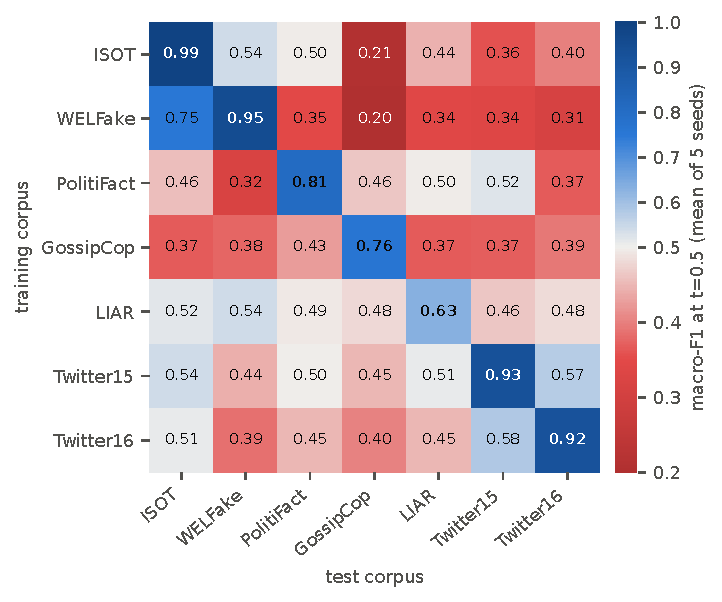
\includegraphics[width=0.48\linewidth]{fig_heatmap_f1}\hfill
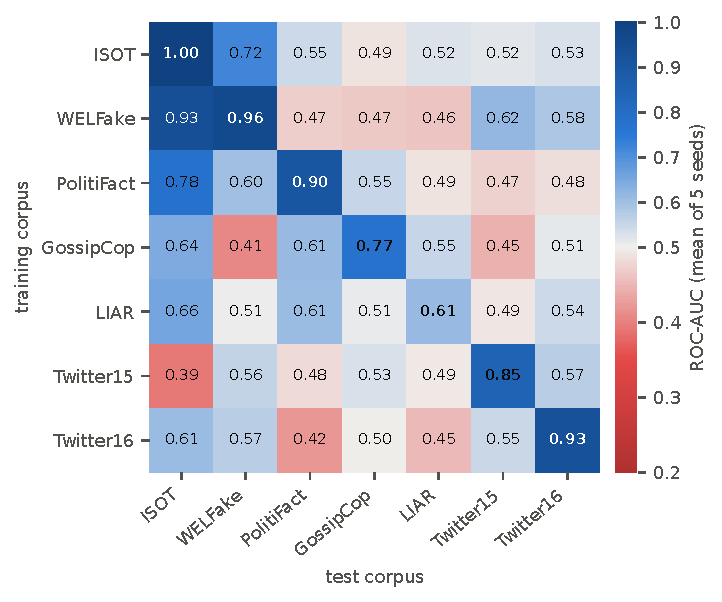
\includegraphics[width=0.48\linewidth]{fig_heatmap_auc_roberta}
\caption{Left: macro-F1 at $t=0.5$ for \textsc{tfidf-lr}. Right: ROC-AUC for frozen RoBERTa representations on the 1{,}500-item subsets.}
\end{figure}
\begin{figure}[h]
\centering
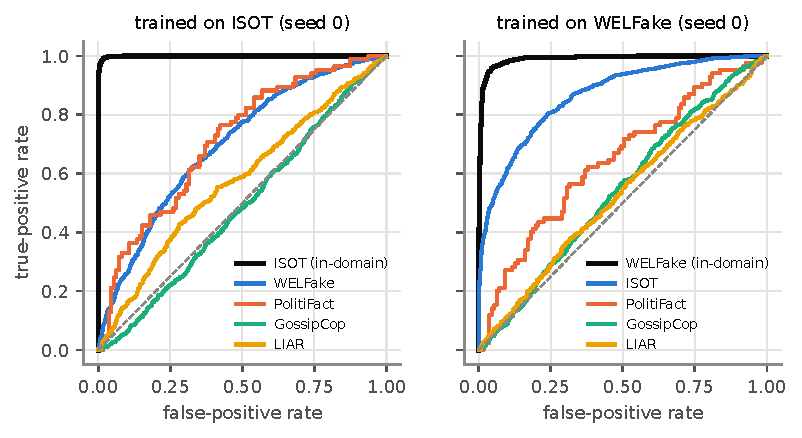
\includegraphics[width=0.9\linewidth]{fig_roc}
\caption{ROC curves (seed 0) for models trained on ISOT and WELFake, in-domain and on four other corpora.}
\end{figure}
\begin{figure}[h]
\centering
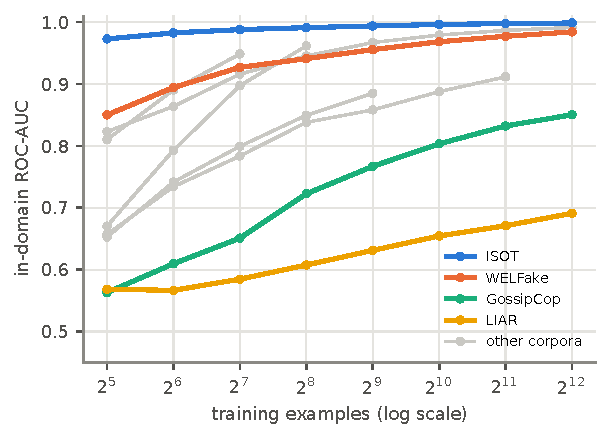
\includegraphics[width=0.48\linewidth]{fig_learning_curve}\hfill
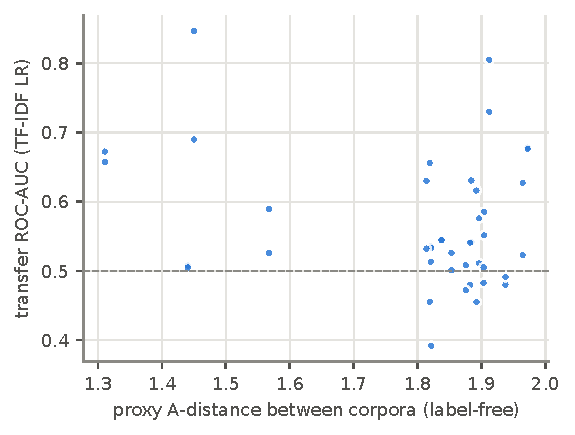
\includegraphics[width=0.48\linewidth]{fig_pad}
\caption{Left: in-domain learning curves. Right: proxy $\mathcal{A}$-distance between corpora against transfer AUC (Spearman $\rho=\PADrho$).}
\end{figure}
\begin{figure}[h]
\centering
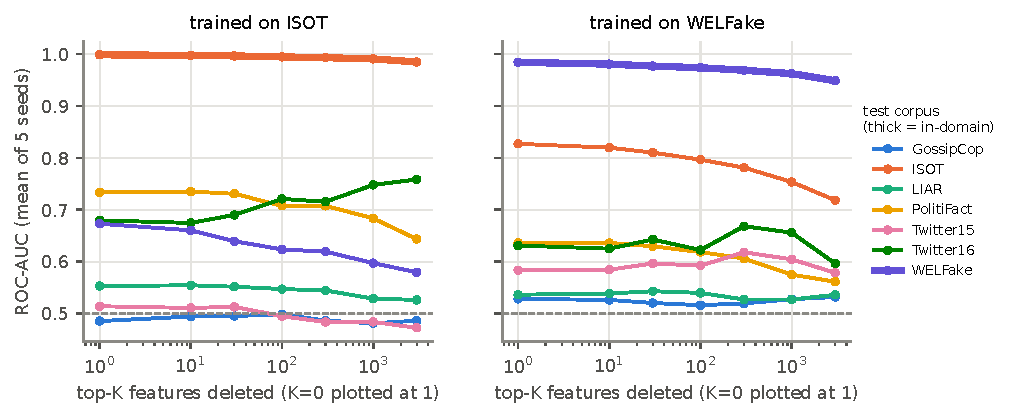
\includegraphics[width=0.9\linewidth]{fig_topk}
\caption{Top-$K$ feature deletion: in-domain and transfer AUC as the $K$ highest-weight features are removed.}
\end{figure}
\begin{figure}[h]
\centering
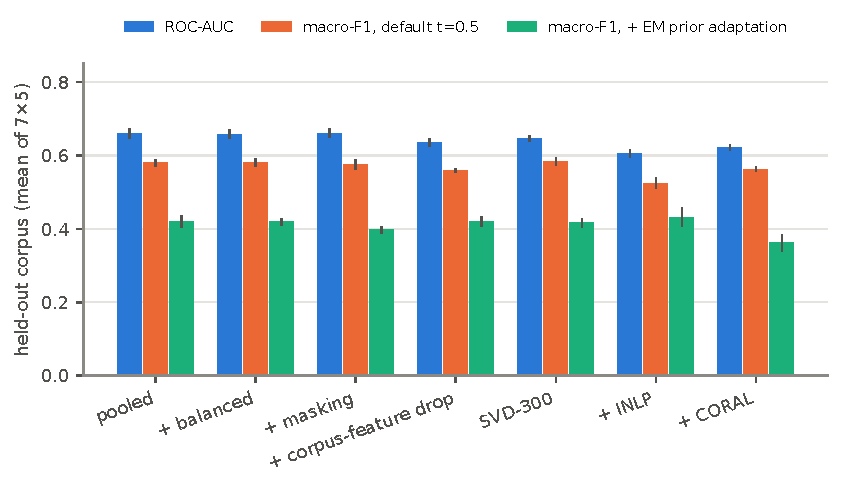
\includegraphics[width=0.9\linewidth]{fig_fix}
\caption{Leave-one-corpus-out repairs: mean over held-out corpora and seeds.}
\end{figure}

\section{Code map}
\small
\begin{tabular}{@{}p{5.6cm}p{10cm}@{}}
\toprule
\texttt{src/prep.py} & corpora, label harmonisation, deduplication, cross-corpus flags \\
\texttt{src/label\_probe.py} & label-direction probes \\
\texttt{src/transfer.py} & transfer matrices (5 models $\times$ 3 regimes $\times$ 5 seeds) \\
\texttt{src/roberta.py} & RoBERTa representations and paired TF-IDF baseline \\
\texttt{src/mechanism.py} & style, group, learning-curve, top-$K$, masking, topic, PAD, weights, vocabulary \\
\texttt{src/fix.py} & leave-one-corpus-out repairs \\
\texttt{src/bangla.py} & BanglaBait replication, leave-one-publisher-out, translate-test \\
\texttt{src/analysis.py}, \texttt{analysis\_extra.py} & aggregation, intervals, decomposition, tests \\
\texttt{src/figures.py}, \texttt{paper\_numbers.py} & every figure, number and table \\
\bottomrule
\end{tabular}

\bibliographystyle{plainnat}
\bibliography{refs}
\end{document}
